%===================================================================================================
% システム設計
%===================================================================================================
\chapter{ステレオカメラを用いた位置同定}
本章では,位置同定実験を行う際用いられた装置,データ,及びデータの取得法について述べる.

%---------------------------------------------------------------------------------------------------
\section{概要}
本研究の目的は,ステレオカメラを用いた屋内・屋外位置同定である.そこで,ここでは位置同定実験を行う際用いられた装置や,データ,データ取得法について述べる.
本章の流れについて説明すると,まずは提供されたステレオカメラについて述べる.ステレオカメラデータ取得部のシステム構成,キャリブレーション方法,ステレオカメラ画像の特徴などについて説明する.また,今回実験を行う際,用いられたステレオカメラ搭載の実験用台車について述べる.最後に環境地図の生成方法と台車の位置計測法について述べる.なお,本研究では地図データや計測データはすべてPTX形式で表現,保存されている..
\newpage
%---------------------------------------------------------------------------------------------------
\section{ステレオカメラ}

\subsection{ステレオカメラデータ取得部のシステム構成}
ステレオカメラデータ取得部のシステム構成説明の前に,ステレオカメラについて述べる.本研究で用いたステレオカメラはセンサーフォーマット1/1.8インチで有効画像数が1280*640である.レンズの水平視野角89°,焦点距離3.5mm,取得レート15fps,それに,絞りF4.0である物となる.ステレオカメラ2つの間は300mmに置いて撮ったデータはMRPT改造 Rawlog-Grabberというキャッチャーソフトにより左右のJPG画像ができる.OpenCV(C++)視差画像生成ソフトを用いて距離画像(Depth画像)とカラー画像(RGB画像)を生成する.このときキャリブレーションソフトによるステレオカメラの歪・平行化補正が行われる.最後に,MRPT改造 Kinect-3D-SLAMというVisual Odometoryソフトを用いることにより,PointCloudの3次元表示ができる.今回用いたステレオカメラを図{\ref{ステレオカメラ}}に表す.また,図{\ref{システム構成}}にステレオカメラデータ取得部のシステム構成の流れを表す.

\vspace{5mm}
\begin{figure}[htbp]
  \begin{center}
   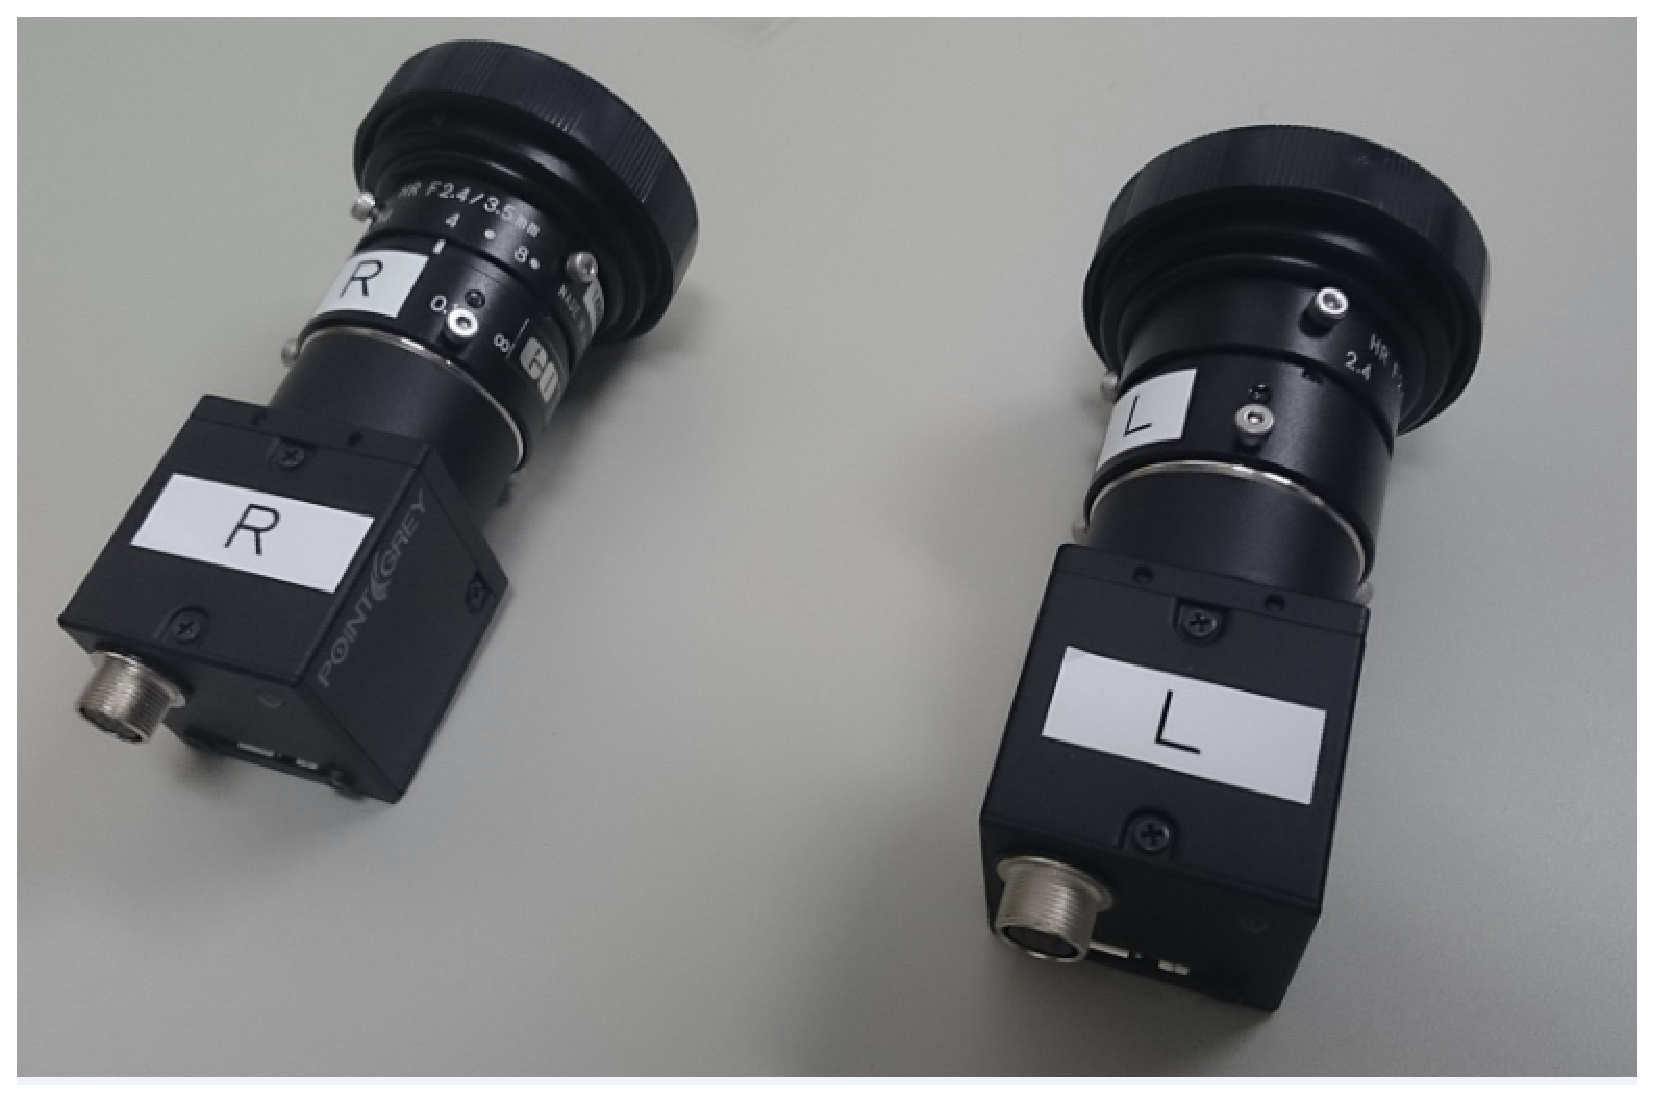
\includegraphics[height=60mm]{figure/ステレオカメラ.eps}
   \caption{ステレオカメラ}
   \label{ステレオカメラ}
  \end{center}
\end{figure}

\newpage

\vspace{5mm}
\begin{figure}[htbp]
  \begin{center}
   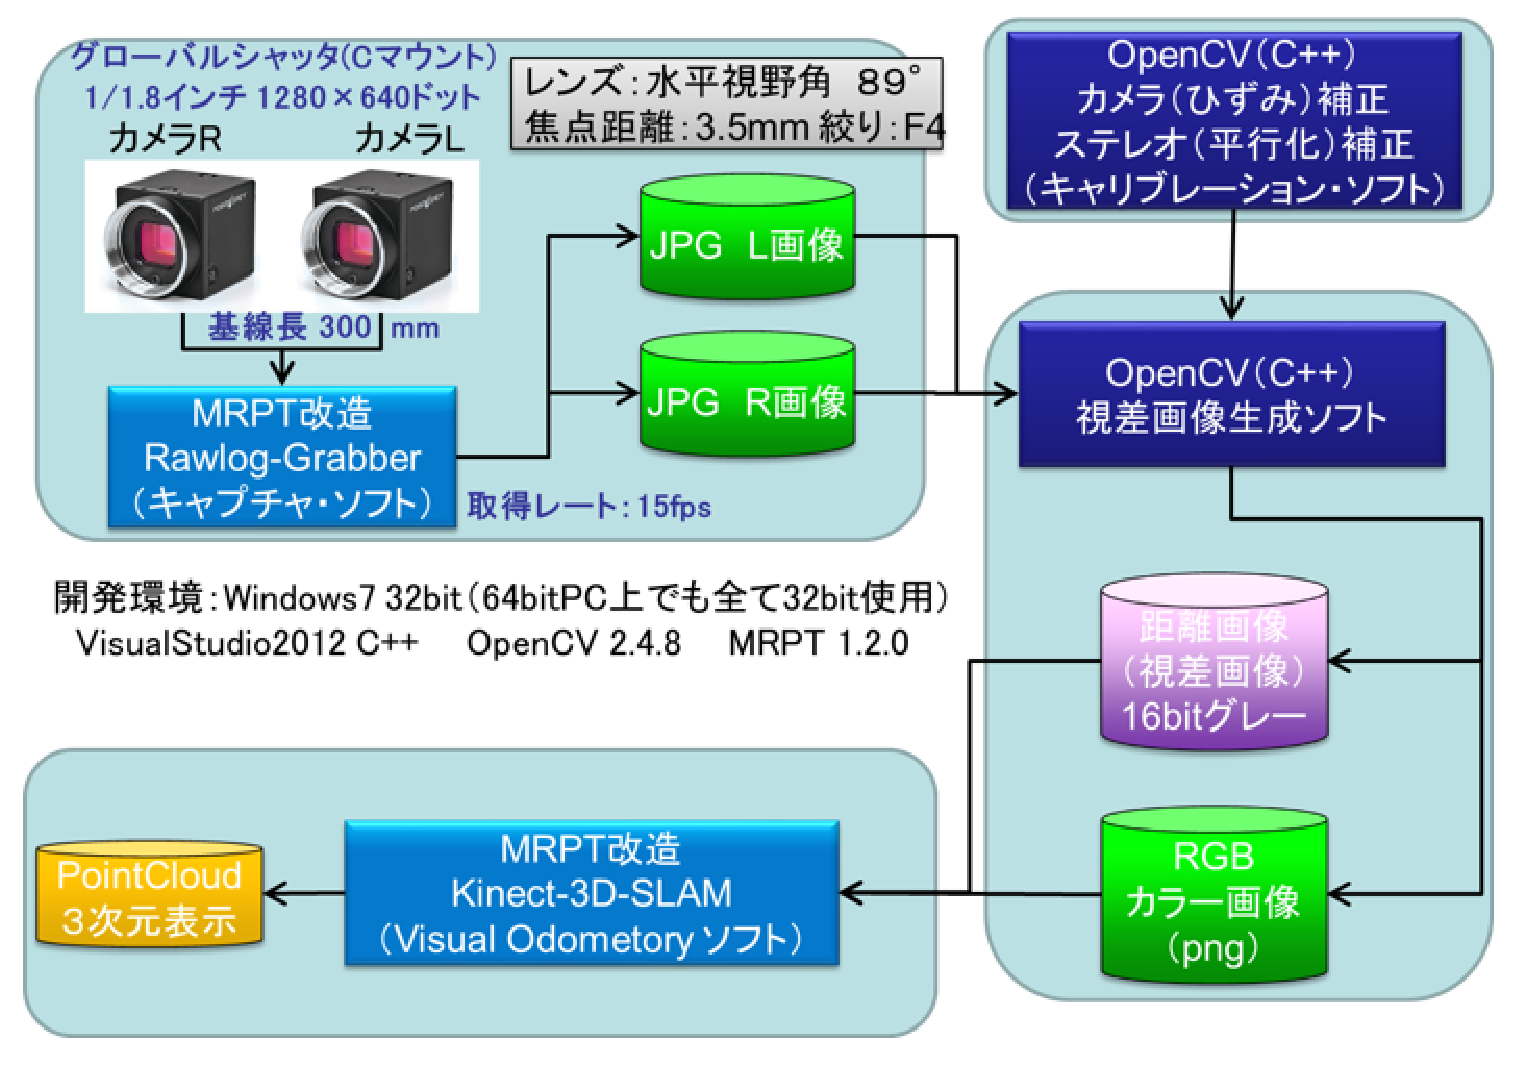
\includegraphics[height=80mm]{figure/システム構成.eps}
   \caption{システム構成}
   \label{システム構成}
  \end{center}
\end{figure}

\subsection{キャリブレーション}
前述した通り,ステレオカメラの歪・平行化補正を行うためにはキャリブレーションを行う必要がある.そこで,キャリブレーションの手順について述べる.
キャリブレーションする前にカメラ準備が要る.カメラ準備の手順は下のようになる.

\begin{enumerate}
 \item ステレオカメラにレンズを付ける.
 \item ステレオカメラをプレートにつけ,三脚に建てる.
 \begin{itemize}
      \item キャリブレーションする際は,ステレオカメラを三脚につける必要があるため,プレートが要る.プレートのイメージを図3.3に表す.また,図{\ref{プレート}}に実際のプレート付きのステレオカメラを表す.
 \end{itemize}

\begin{figure}[htbp]
  \begin{center}
   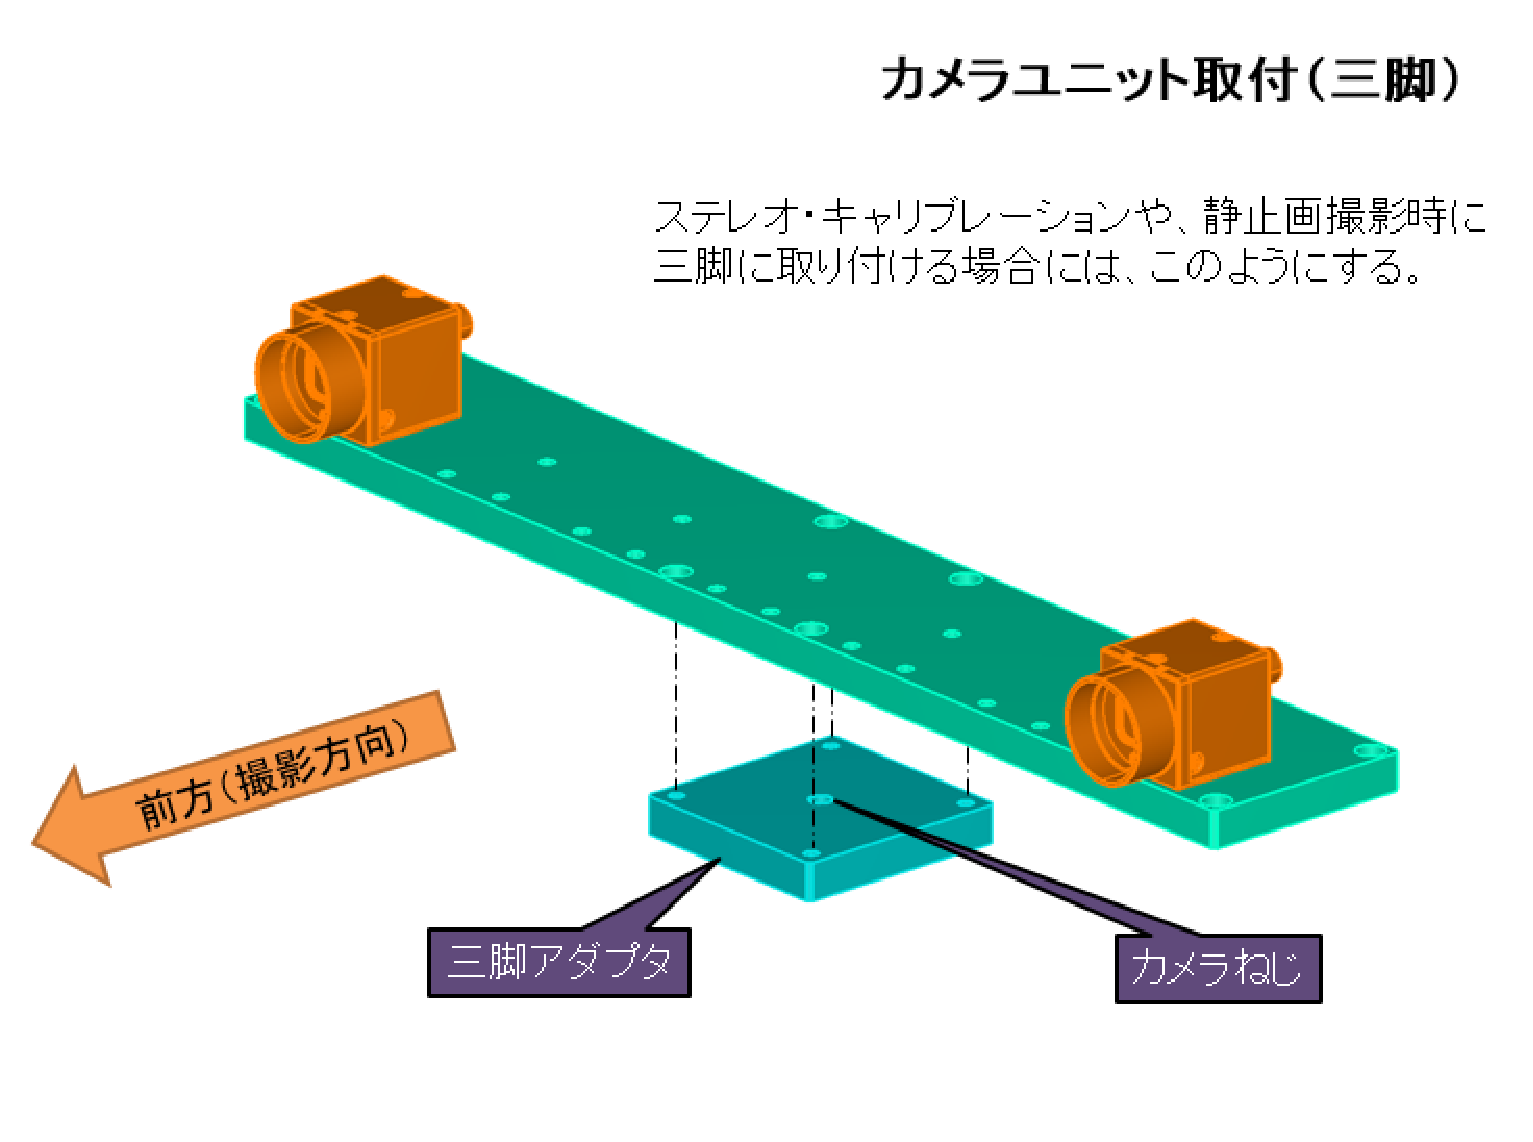
\includegraphics[height=80mm]{figure/プレートイメージ.eps}
   \caption{プレートイメージ}
   \label{プレートイメージ}
  \end{center}
\end{figure}
\begin{figure}[htbp]
  \begin{center}
   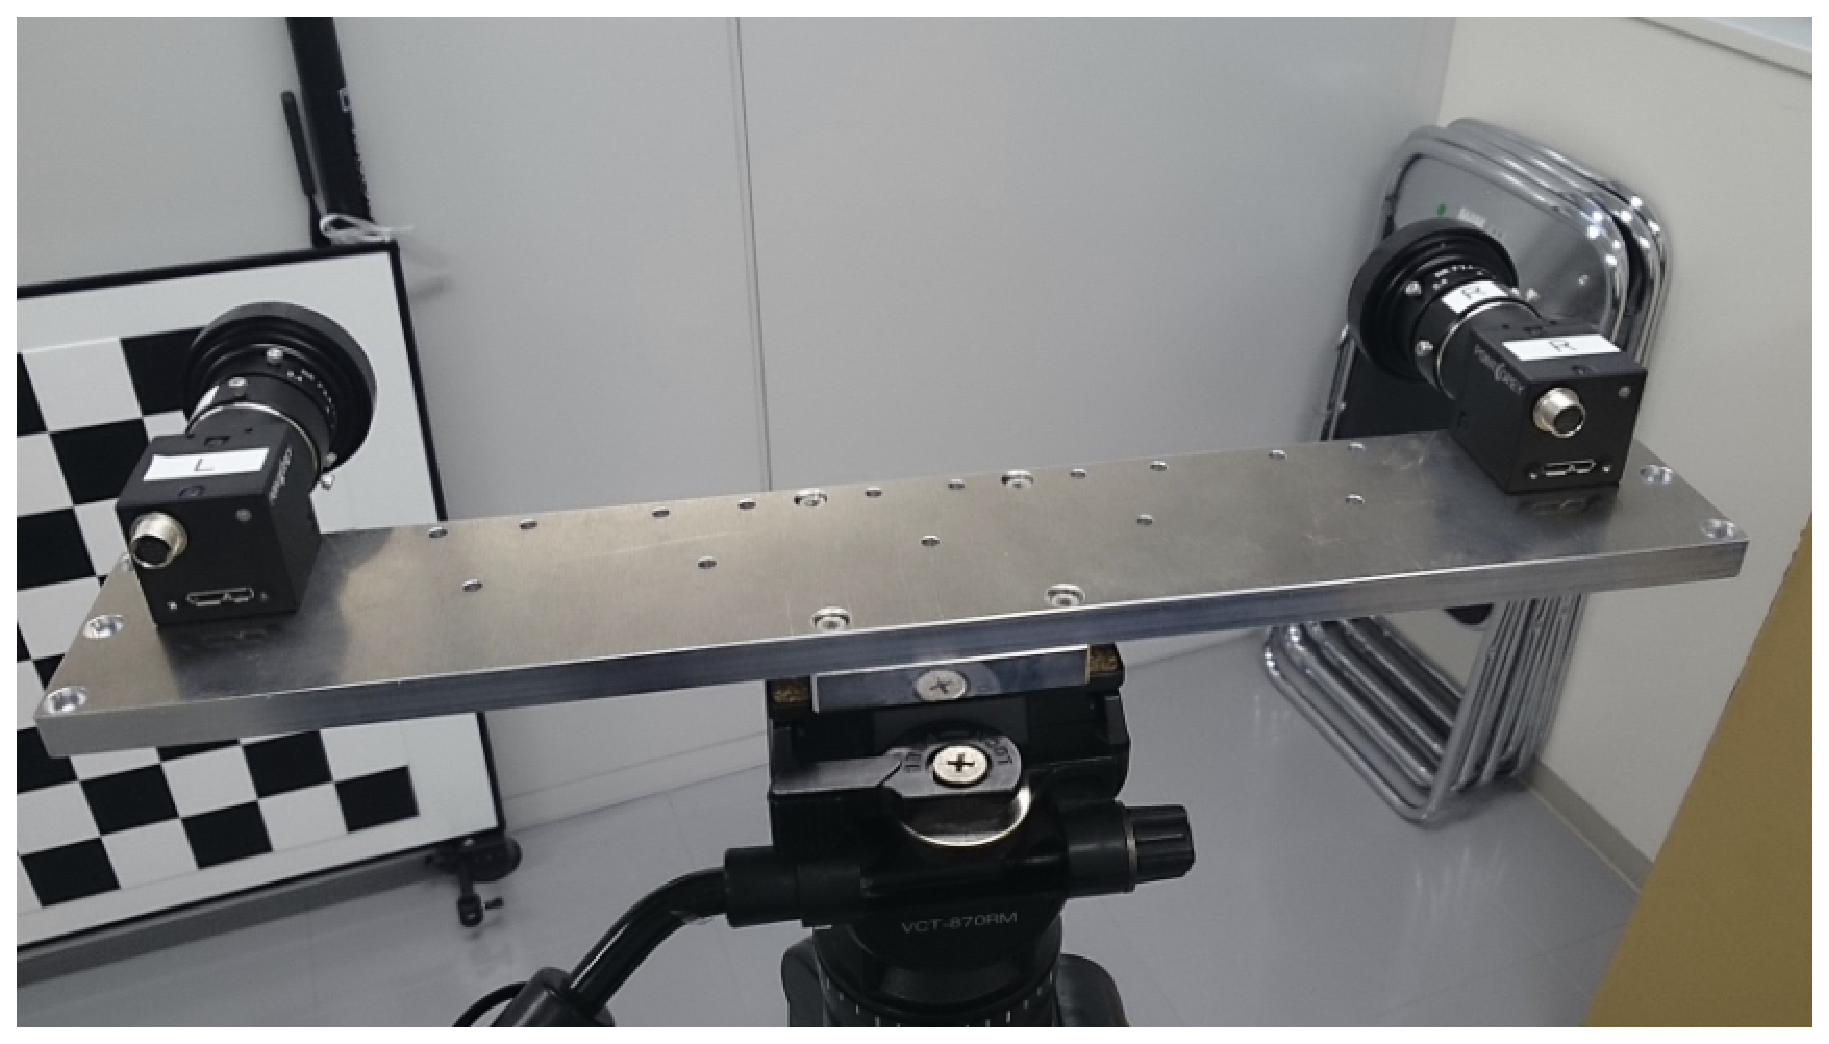
\includegraphics[height=80mm]{figure/プレート.eps}
   \caption{プレート}
   \label{プレート}
  \end{center}
\end{figure}
 \item USB3.0ケーブルをカメラとPCに繋げる.
  \begin{itemize}
      \item このステレオカメラはデータをUSB3.0ケーブルを用いてPCに通す.図3.5にキャリブレーション際の設置イメージを表す.
\begin{figure}[htbp]
  \begin{center}
   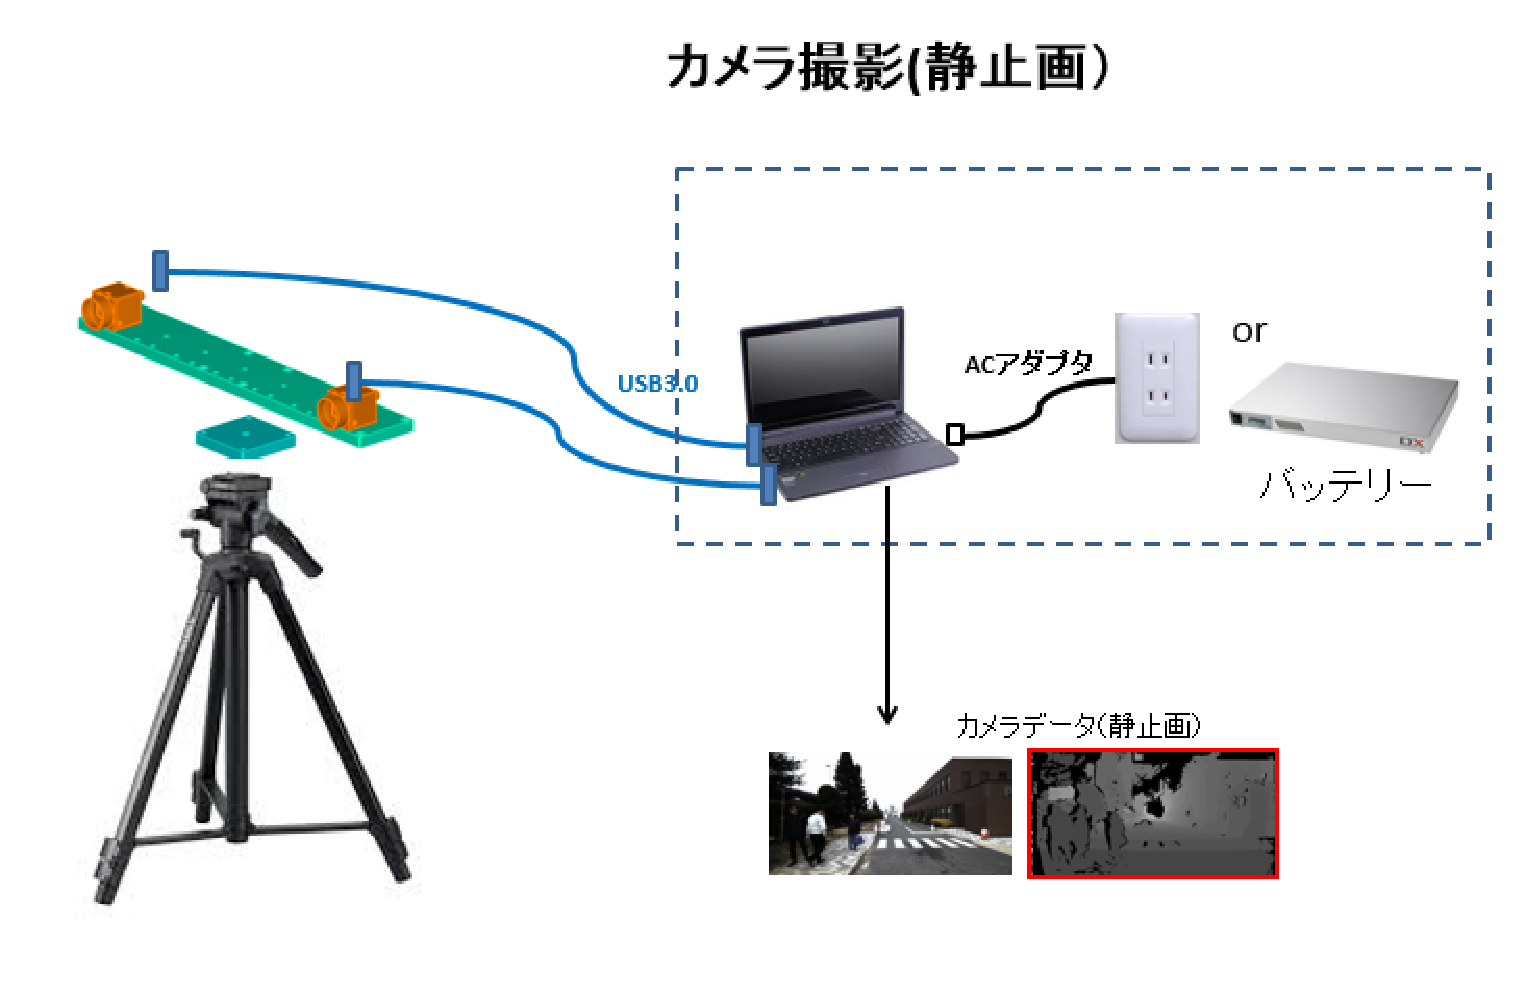
\includegraphics[height=80mm]{figure/設置イメージ.eps}
   \caption{設置イメージ}
   \label{設置イメージ}
  \end{center}
\end{figure}
 \end{itemize}
 \item キャリブレーション撮影ツールを起動し,ステレオカメラの左右確認及びフォーカス調整をする.
\end{enumerate}

ここまでが,カメラ準備の手順となり,キャリブレーションの手順は下のようになる.

\begin{enumerate}
\item キャリブレーションボードを設置して,キャリブレーション撮影ツールを起動する.
\begin{itemize}
\item キャリブレーションボードを図{\ref{キャリブレーションボード}}に,構成を以下に示す.
\item 小アクリル板\\
  各90mm x 90mm, 厚み2.0mm、2色(白黒) 各44枚
\item 大アクリル板\\
  A0サイズ(841mm x 1189mm)\\
  縦8枚 x 横11枚= 合計88枚(720mm x 990mm)の小アクリル板を、大きなアクリル板上の\\
  中央に白黒交互に貼り合わせする.
\item 補強として、枠が小アクリル板と重ならないようにするため,外側に枠を取り付けする.
\begin{figure}[htbp]
  \begin{center}
   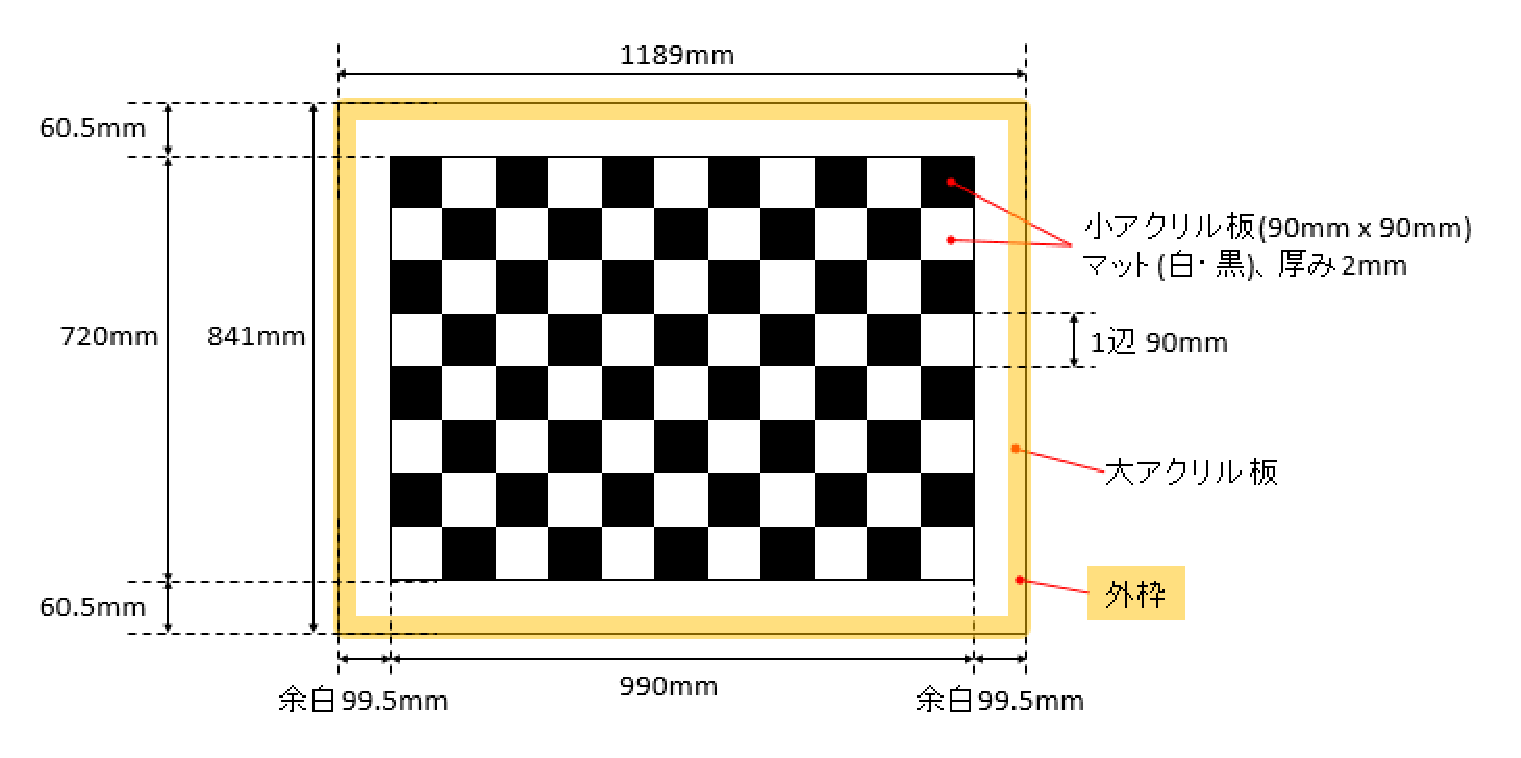
\includegraphics[height=80mm]{figure/キャリブレーションボード.eps}
   \caption{キャリブレーションボード}
   \label{キャリブレーションボード}
  \end{center}
\end{figure}
\end{itemize}

\vspace{15mm}
\item ボードの上(三脚高さ:1.5m,ボードの高さ:1m)\\
->左(カメラを左に傾け),左(右に傾け),中央,右(左に傾け),右(右に傾け)\\

ボードの中央\\
->左(ボードからの距離:50cm),左(ボードからの距離:100cm),中央(ボードからの距離:50cm)\\
中央(ボードからの距離:100cm),右(ボードからの距離:50cm), 右(ボードからの距離:100cm)\\

ボードの下(三脚高さ:0.5m,ボードの高さ:1.7m)\\
->左(左に傾け),左(右に傾け),中央,右(左に傾け),右(右に傾け)\\

暗室で照明が安定なところで総16パターン撮影を行う.図3.7,図3.8にキャリブレーション撮影例を表す.

\begin{figure}[htbp]
  \begin{center}
   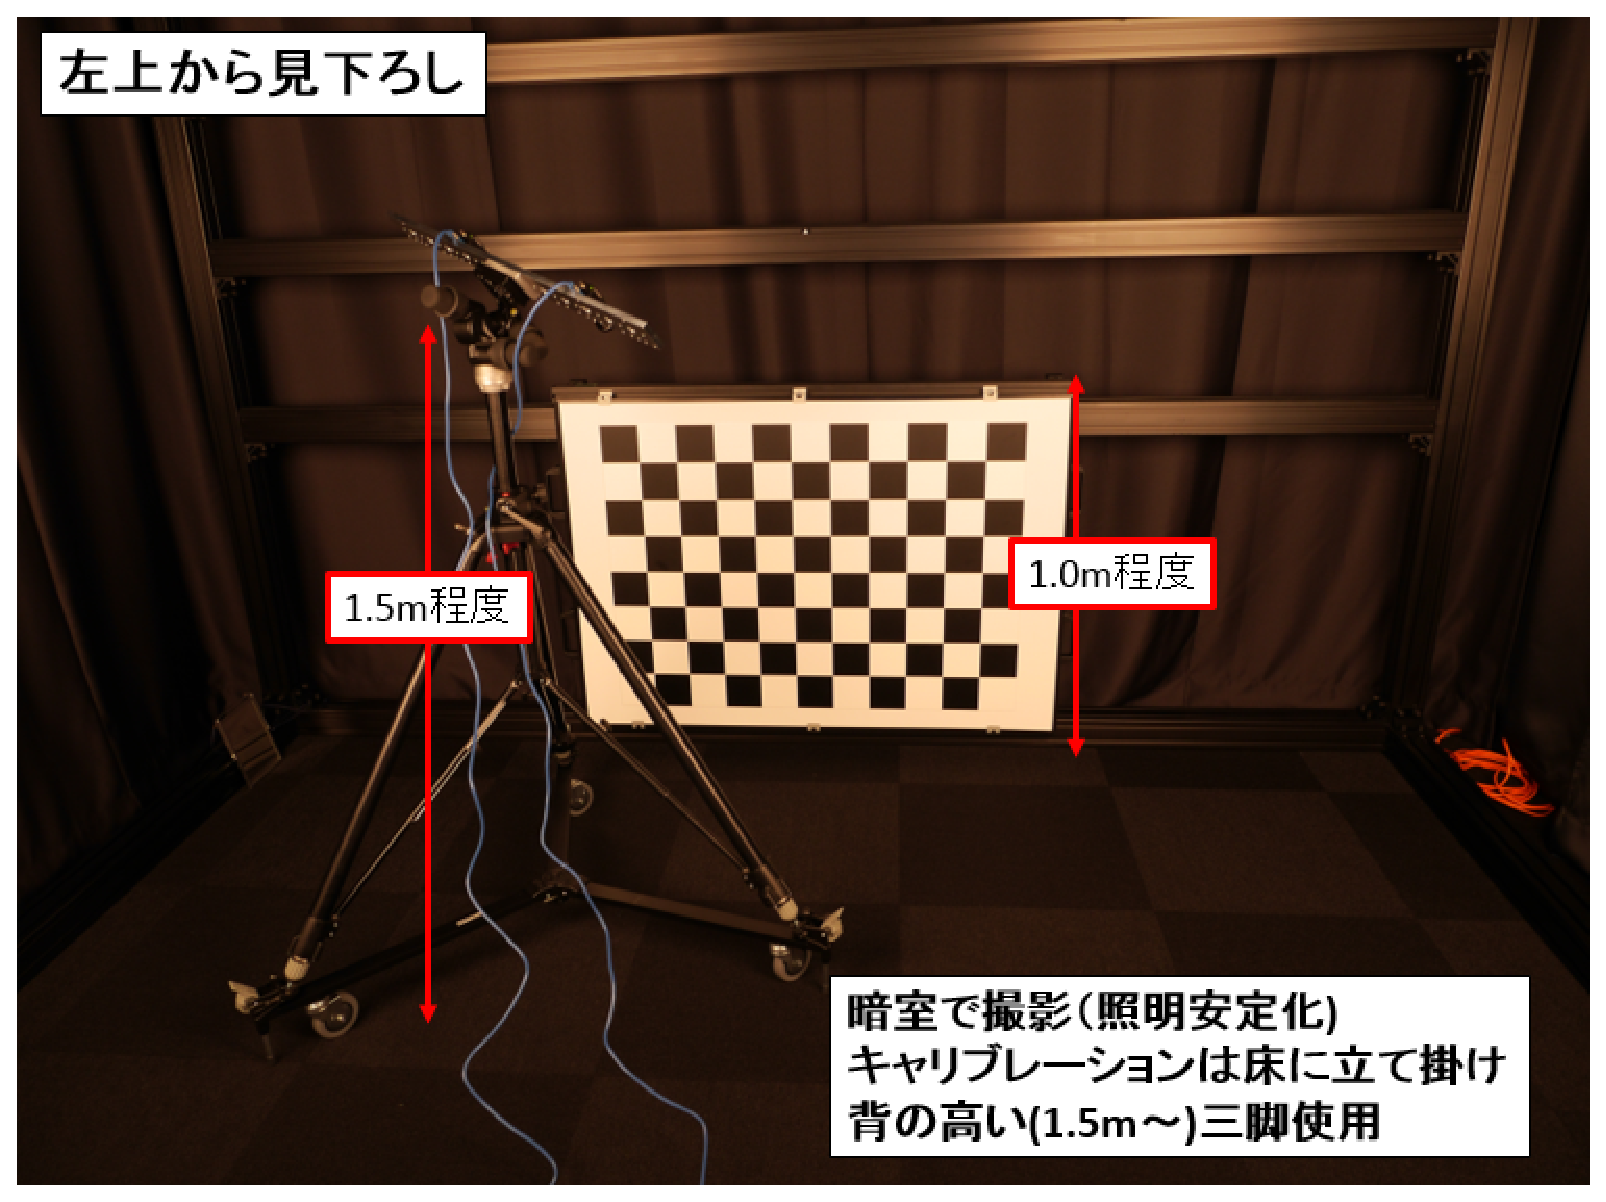
\includegraphics[height=80mm]{figure/caribration1.eps}
   \caption{キャリブレーション撮影例1}
   \label{caribration1}
  \end{center}
\end{figure}

\begin{figure}[htbp]
  \begin{center}
   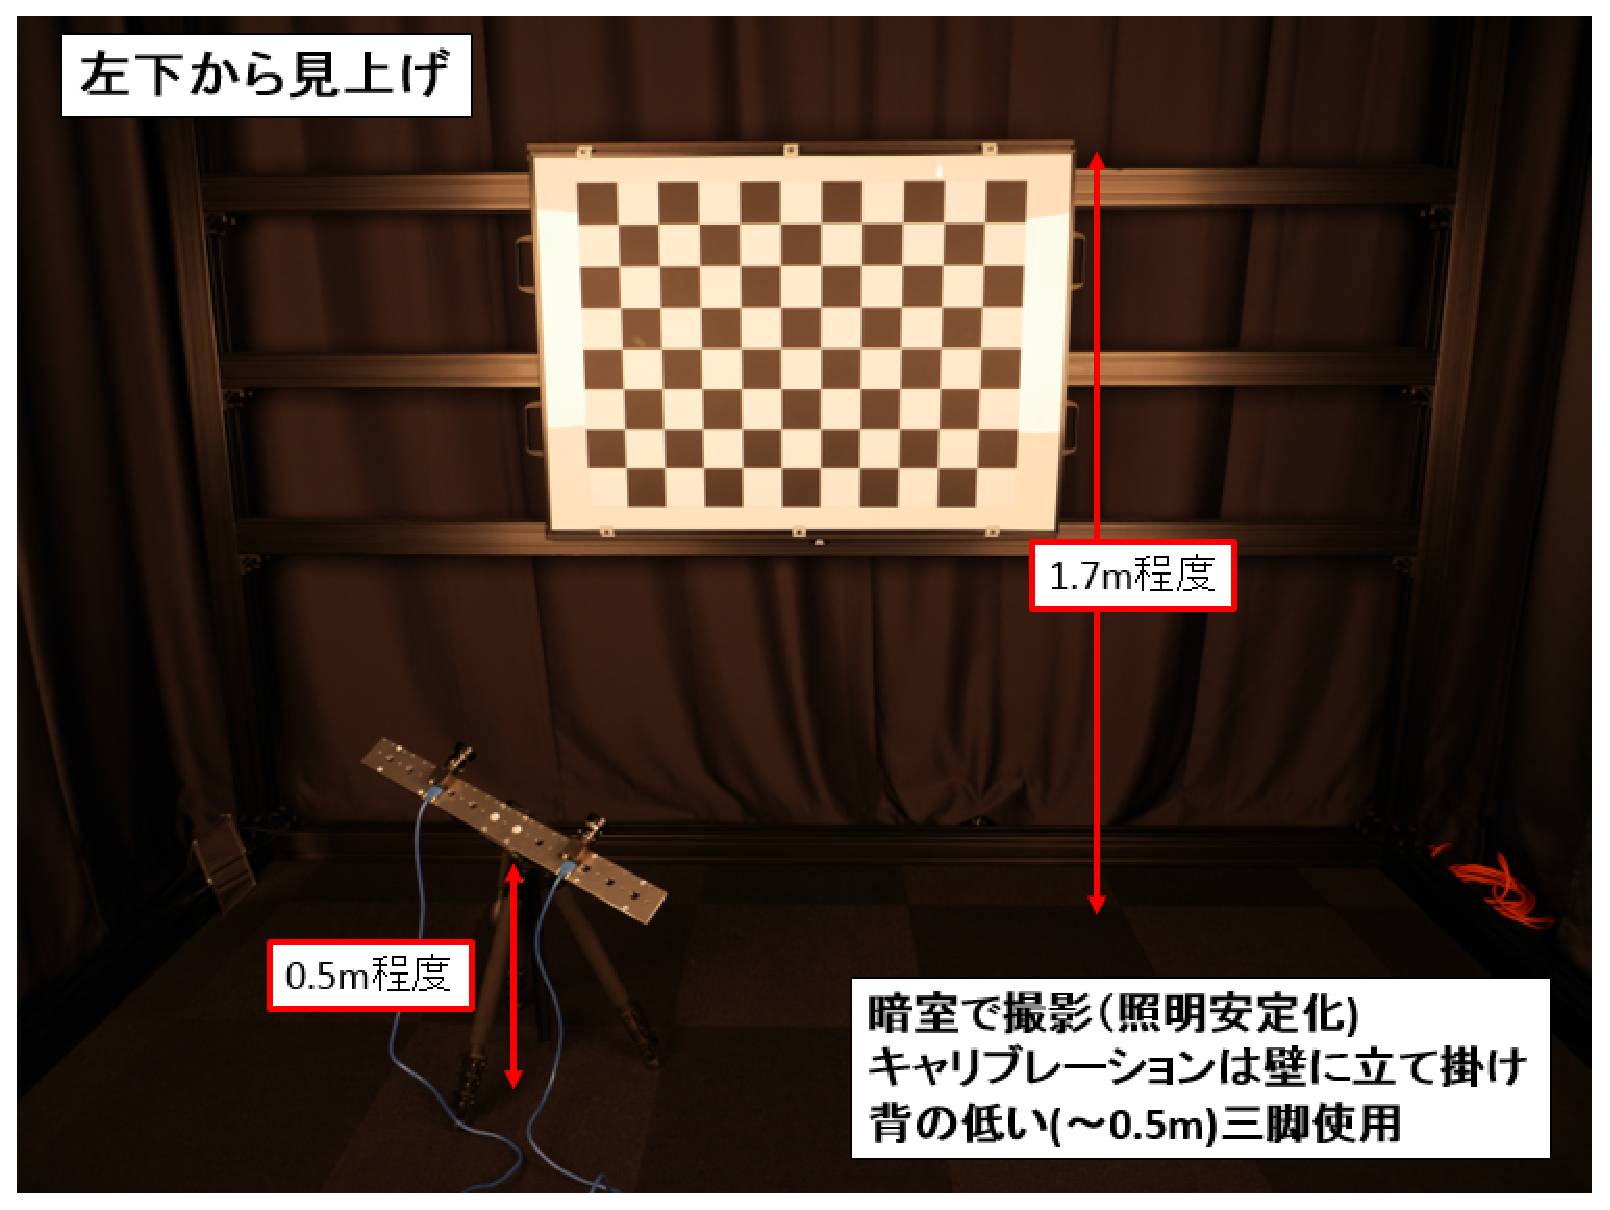
\includegraphics[height=80mm]{figure/caribration2.eps}
   \caption{キャリブレーション撮影例2}
   \label{caribration2}
  \end{center}
\end{figure}

\item キャリブレーション実行ツールを起動する.

\end{enumerate}
\newpage

\subsection{ステレオ画像の特徴}
ステレオ画像とは, 景色や物などを2つの視点から撮った画像を左右に並べたものである.2つの視点はそれぞれ右目と左目で見たように水平方向にお互いに少し離れている.2つの視点から各々見られる画像は少しズレがあるが,それを視差という.左右の視点間の距離と対応点の視差から,奥行きが計算できる.

ステレオカメラから得られる距離画像(ステレオ画像)と,RGB-Dカメラから得られる距離画像(RGB-D画像)を図3.9,図3.10に表す.各々の図はMeshLabを用いてPTX化されたデータを表示したもので,ステレオ画像のデータを安定に撮れるようにするため,壁にテクスチャーを貼った状態である.\\

\begin{figure}[ht]
  \begin{center}
   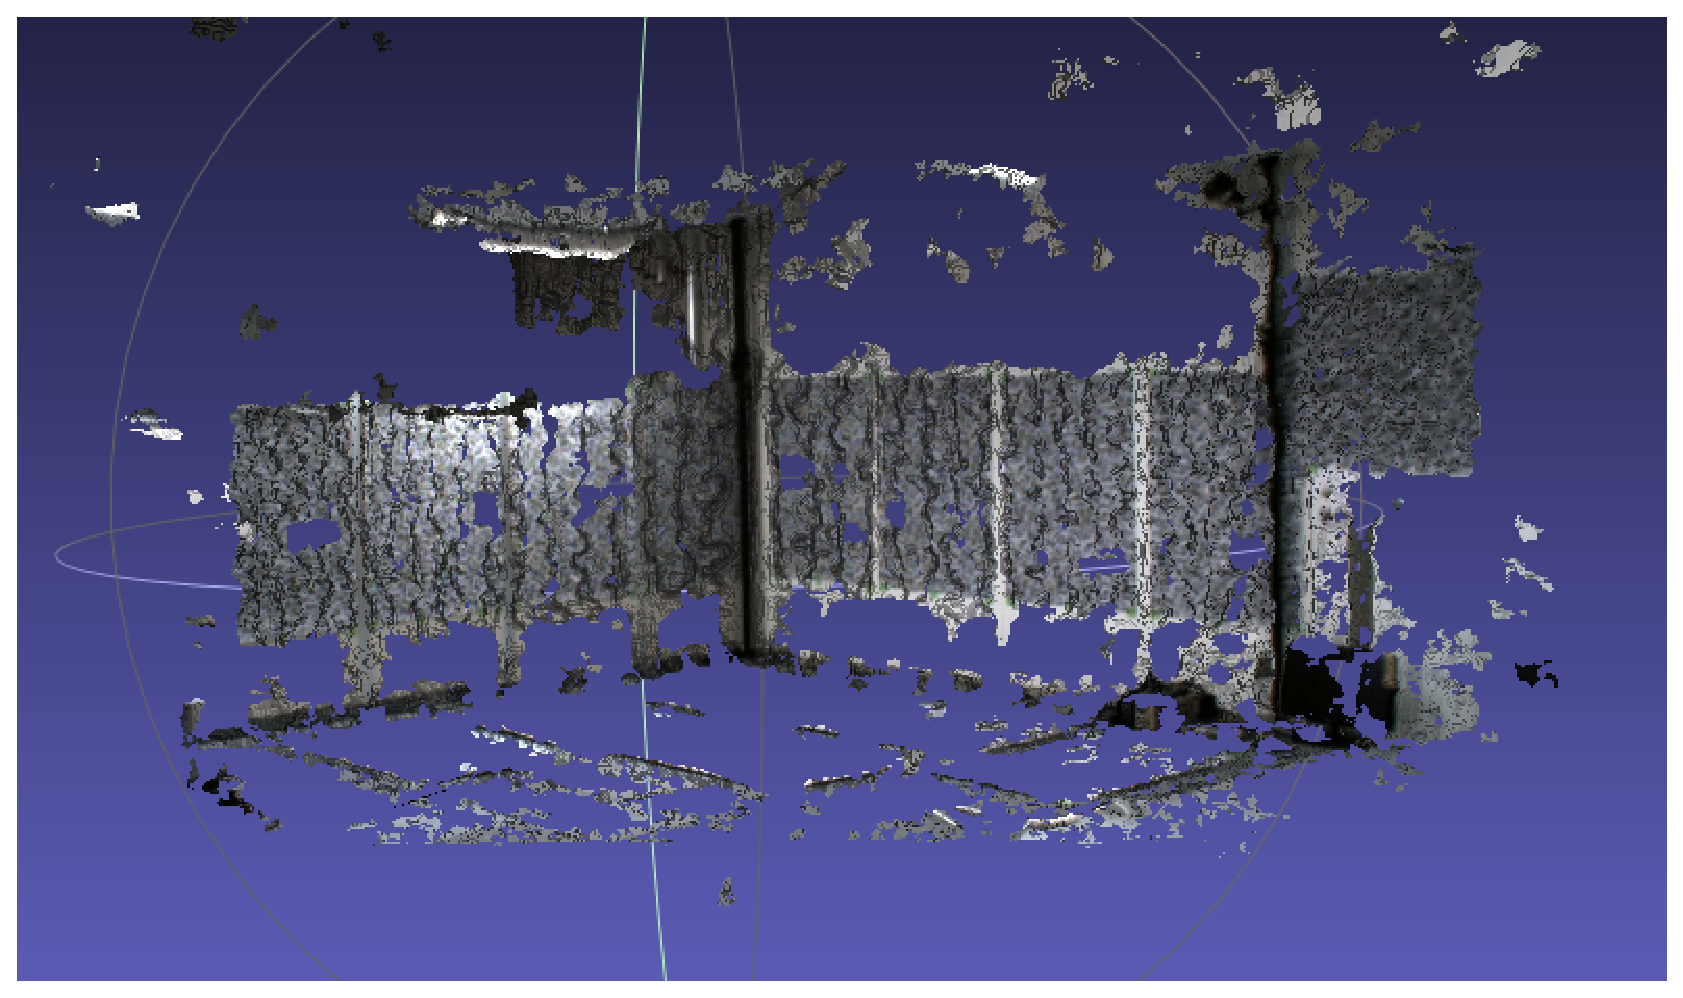
\includegraphics[height=50mm]{figure/ステレオ画像.eps}
   \caption{ステレオ画像}
   \label{ステレオ画像}
  \end{center}
\end{figure}

\begin{figure}[h]
  \begin{center}
   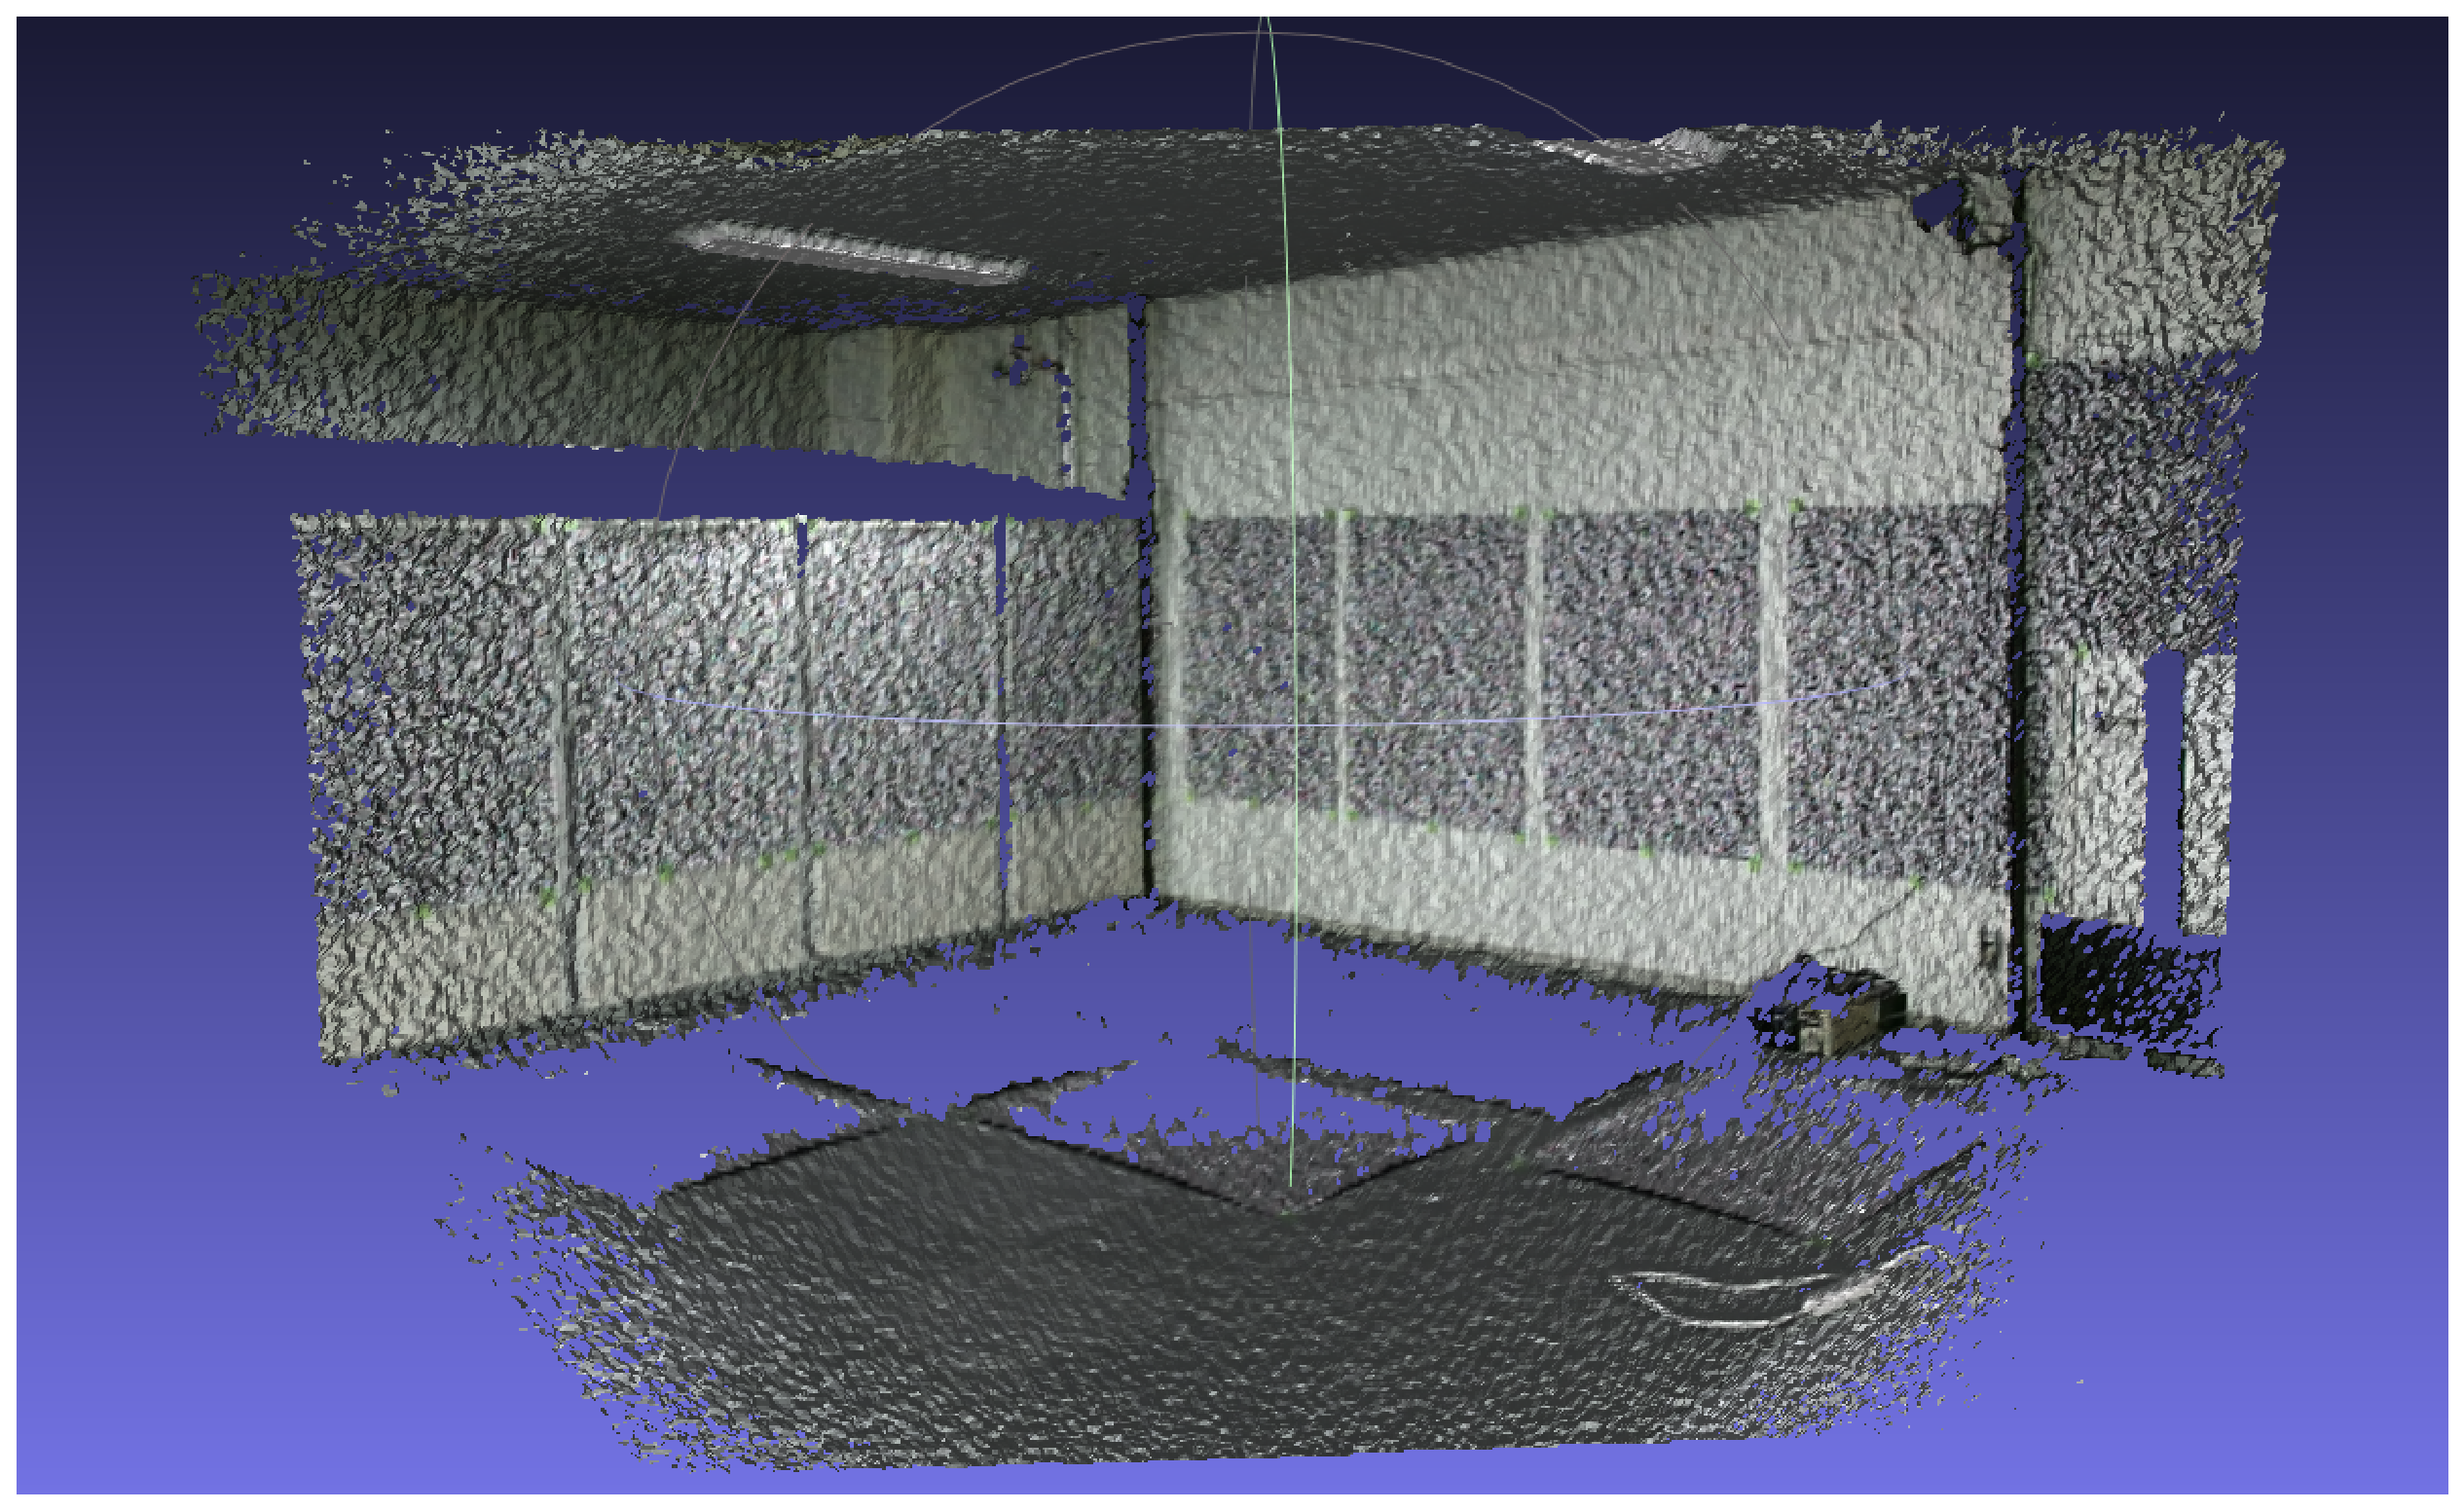
\includegraphics[height=50mm]{figure/RGB-D画像.eps}
   \caption{RGB-D画像}
   \label{RGB-D画像}
  \end{center}
\end{figure}

\newpage

\vspace{5mm}
ステレオ画像とRGB-D画像を比較すると,RGB-D画像の方が精度が良いことが分かる.今回測定したRGB-DカメラはKinect V2である.Kinect V2測定可能距離が最大8mである反面,ステレオカメラは最大20mまで測定可能である.また,Kinect V2の場合,測定可能水平角度が70°であるが,ステレオカメラは89°である.さらに後述のように,Kinect V2は太陽光の影響を受けやすい.このため,屋外ではステレオ画像を用いる方が有利と思われる.

%--------------------------------------------------------------------------------------------------
\section{ステレオカメラを搭載した実験用台車}
本節では,ステレオカメラを搭載する台車について述べる.台車の上にはステレオカメラだけではなくステレオカメラとの比較対象となるKinect V2も載せる.まず,ステレオカメラを台車の上に載せるためにはキャリブレーションで使われたプレートではなく別のプレートにつけなければならない.図3.11に台車用のプレート設計図と図3.12にステレオカメラ取り付けのイメージを表す.また,図3.13に台車全体の取り付けイメージを表す.

\begin{figure}[h]
  \begin{center}
   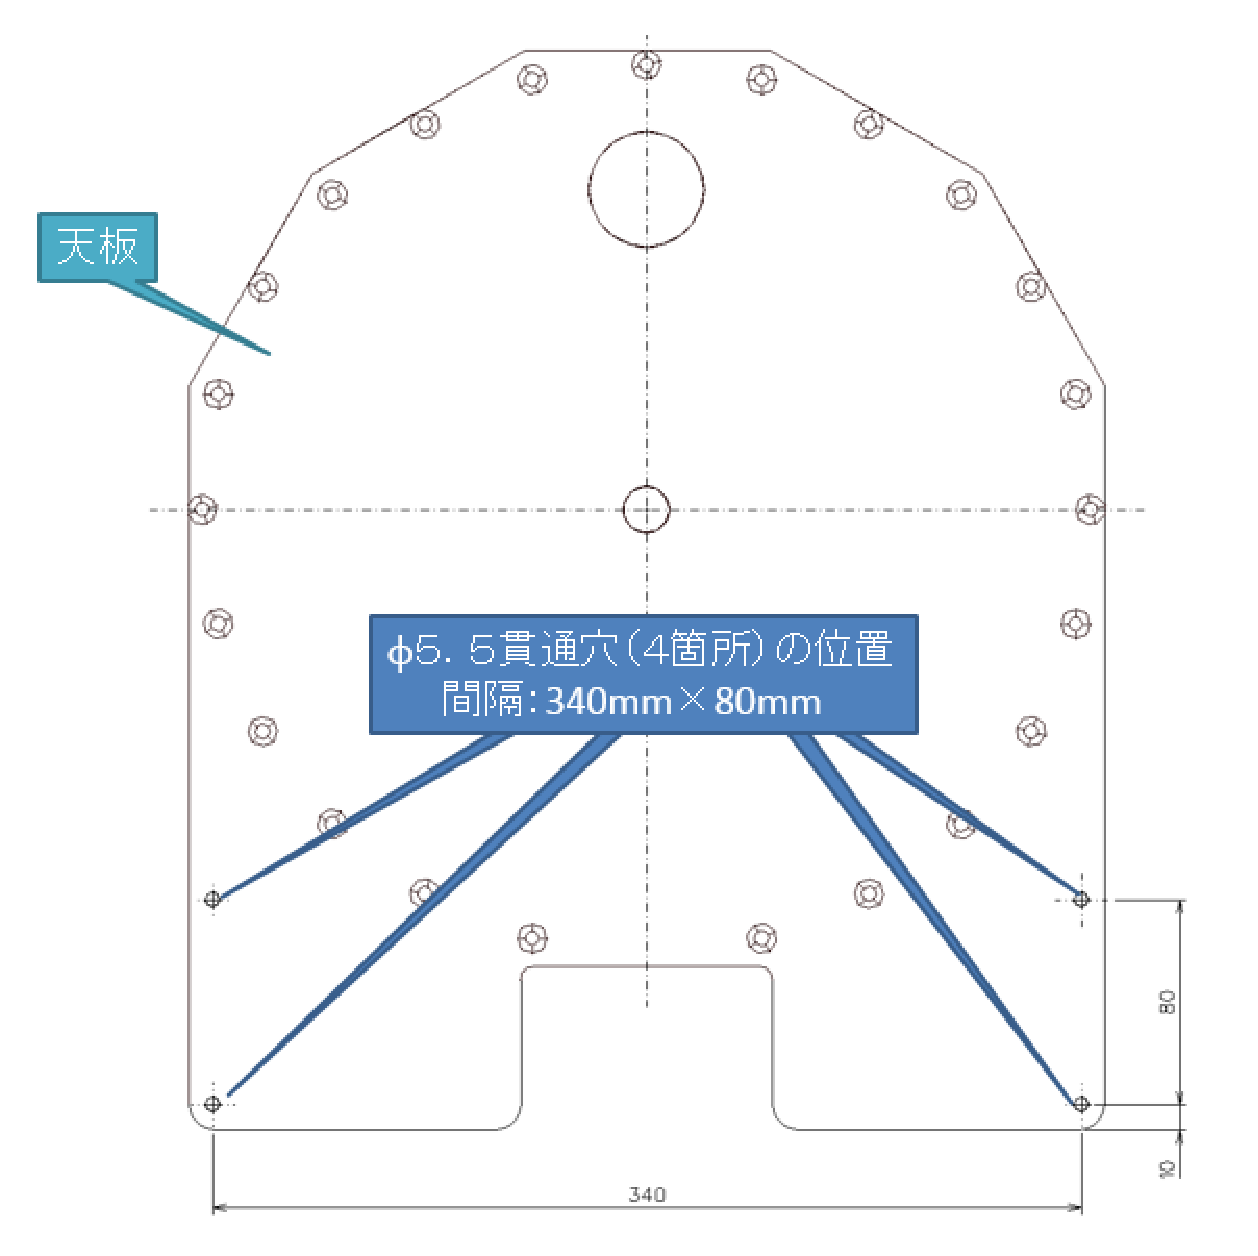
\includegraphics[height=100mm]{figure/台車用のプレート設計図.eps}
   \caption{台車用のプレート設計図}
   \label{台車用のプレート設計図}
  \end{center}
\end{figure}
\newpage
%
\begin{figure}[htbp]
  \begin{center}
   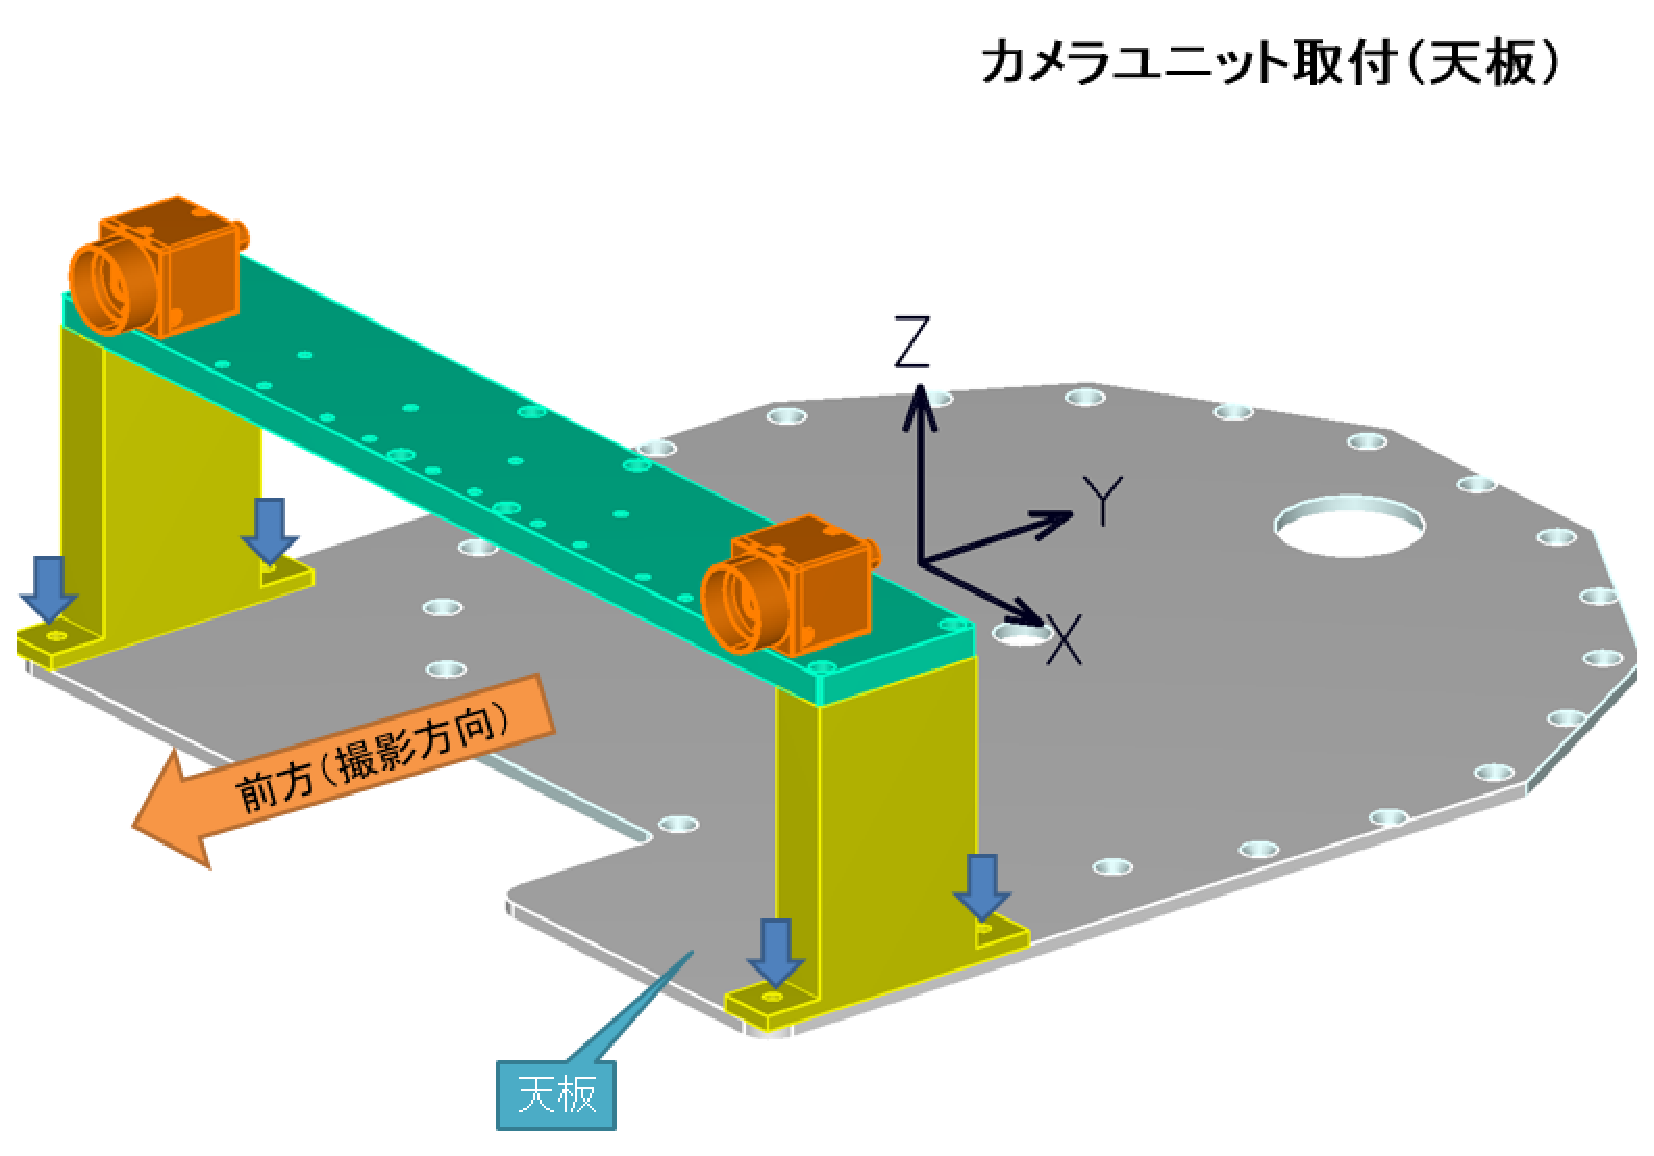
\includegraphics[height=50mm]{figure/ステレオカメラ取り付けのイメージ.eps}
   \caption{ステレオカメラ取り付けのイメージ}
   \label{ステレオカメラ取り付けのイメージ}
  \end{center}
\end{figure}

\begin{figure}[htbp]
  \begin{center}
   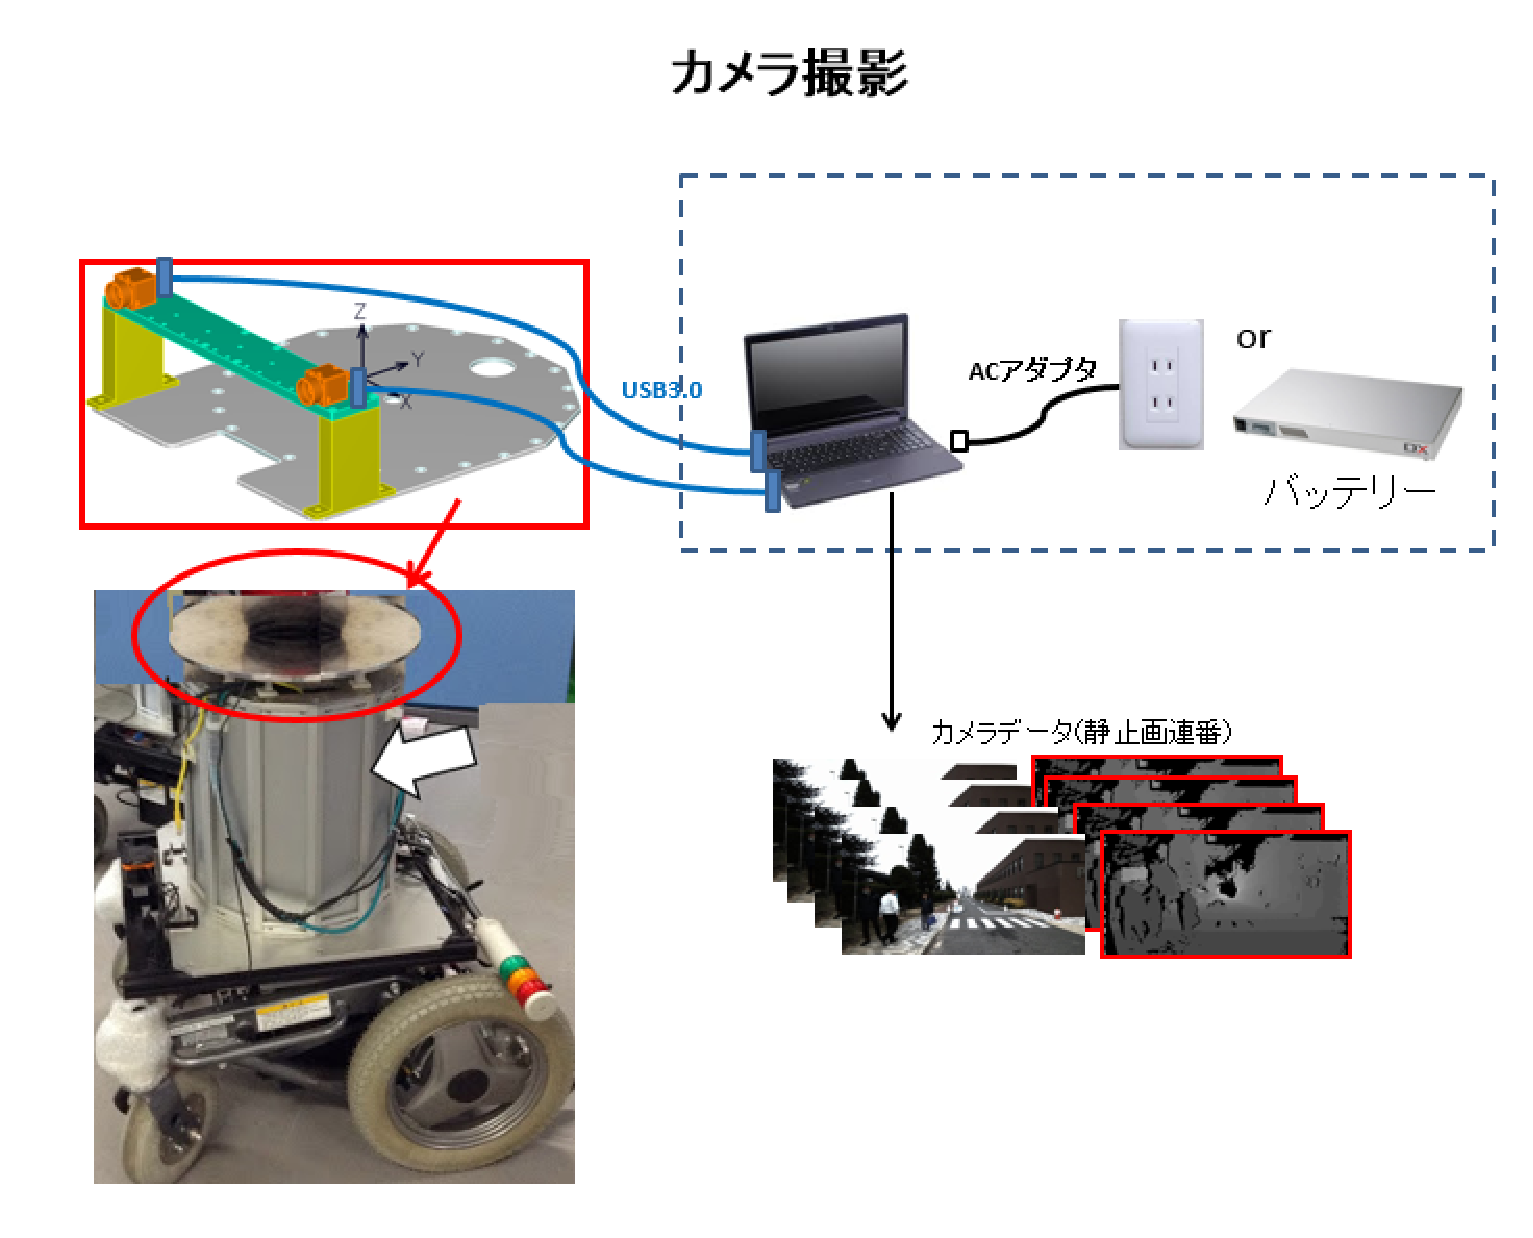
\includegraphics[height=60mm]{figure/台車全体の取り付けイメージ.eps}
   \caption{台車全体の取り付けイメージ}
   \label{台車全体の取り付けイメージ}
  \end{center}
\end{figure}

前述した通り,台車の上にはKinect V2も一緒に載せるが,パソコンと違い,Kinect V2はバッテリが充電式でないためアダプターを切って,バッテリを繋げる作業がいる.図3.14に実際バッテリを繋げたものを表す.図3.14の左からKinect V2のアダプター,DC-DCコンバーター,バッテリとなる.最後に,実際実験に用いる台車のキャッチャーを図3.15に表す.ステレオカメラの上に球を載せる理由は台車の位置計測のためである.


\begin{figure}[htbp]
  \begin{center}
   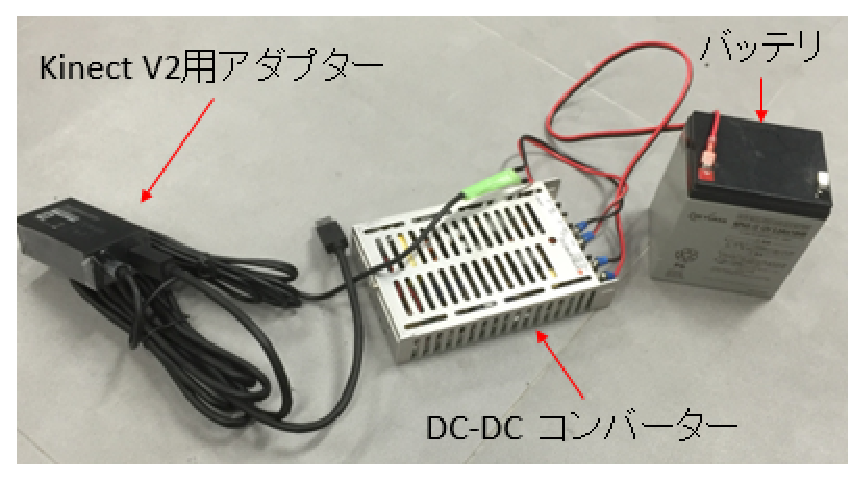
\includegraphics[height=70mm]{figure/battery_kinectV2.eps}
   \caption{バッテリ式Kinect V2}
   \label{battery_kinectV2}
  \end{center}
\end{figure}

\begin{figure}[htbp]
  \begin{center}
   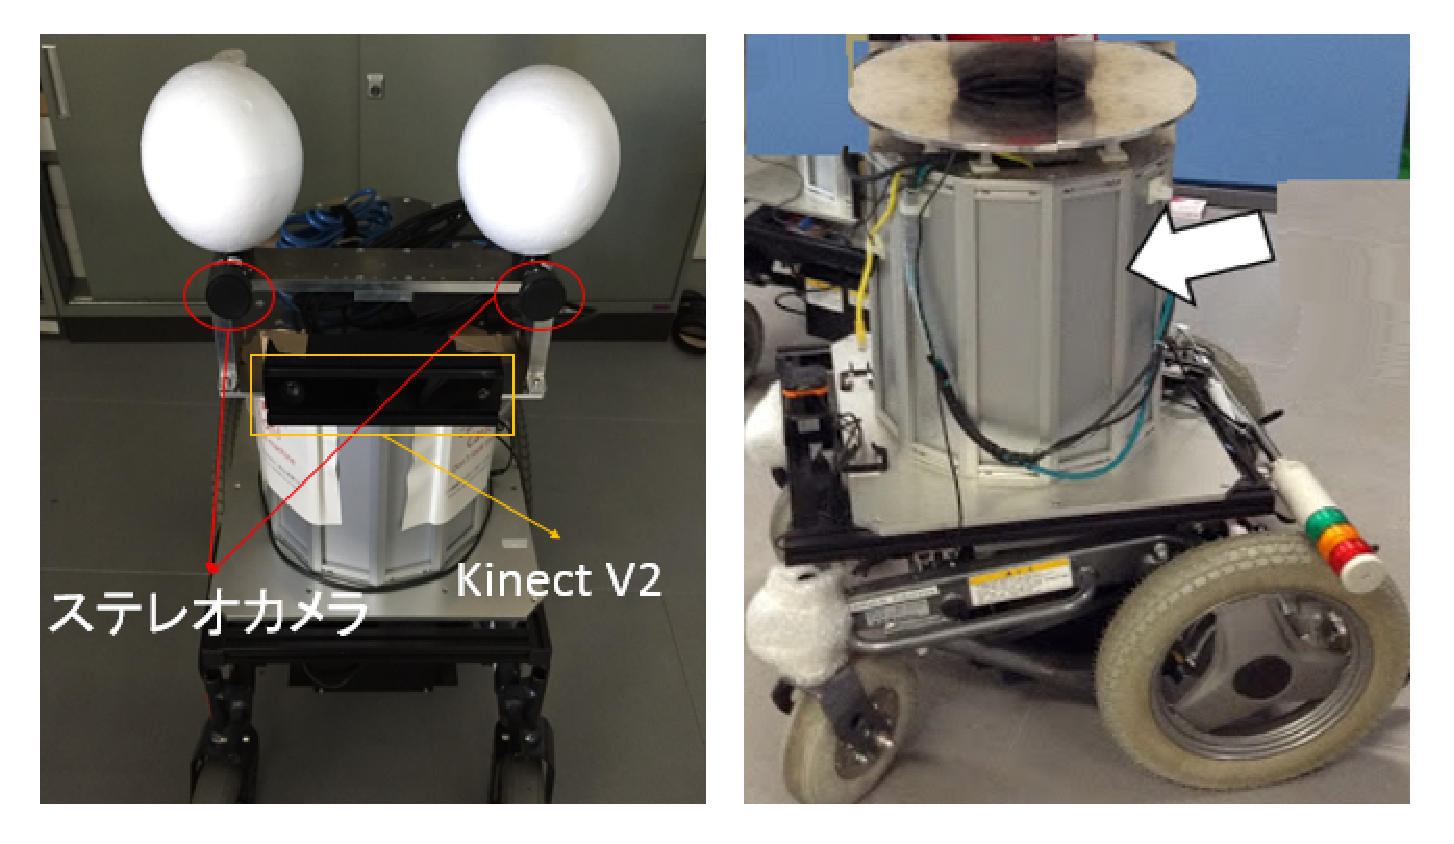
\includegraphics[height=90mm]{figure/台車.eps}
   \caption{台車}
   \label{台車}
  \end{center}
\end{figure}
\newpage

%--------------------------------------------------------------------------------------------------

\section{環境地図}
本節では,ステレオカメラで撮った計測データを用いて位置同定を行う際,必要となる環境地図データの取得法とステレオカメラで撮った場所つまり台車の真値計測法について述べる.

\subsection{環境地図の取得法}
まずは,環境地図の取得法である.環境地図は前述した通り,3次元レーザスキャナFARO Focus 3D (以降FAROと表記)を用いて撮る.FAROは高精度,高密度な点群とカラー画像が取得可能である.またパラメータとしては解像度と品質があり,状況によって調整可能である.解像度は360度を何ポイント計測するかで撮影距離と計測時間に影響がある.品質は同じポイントを何回計測するかでノイズと計測時間に影響がある.図3.16にFAROを表す.

\begin{figure}[htbp]
  \begin{center}
   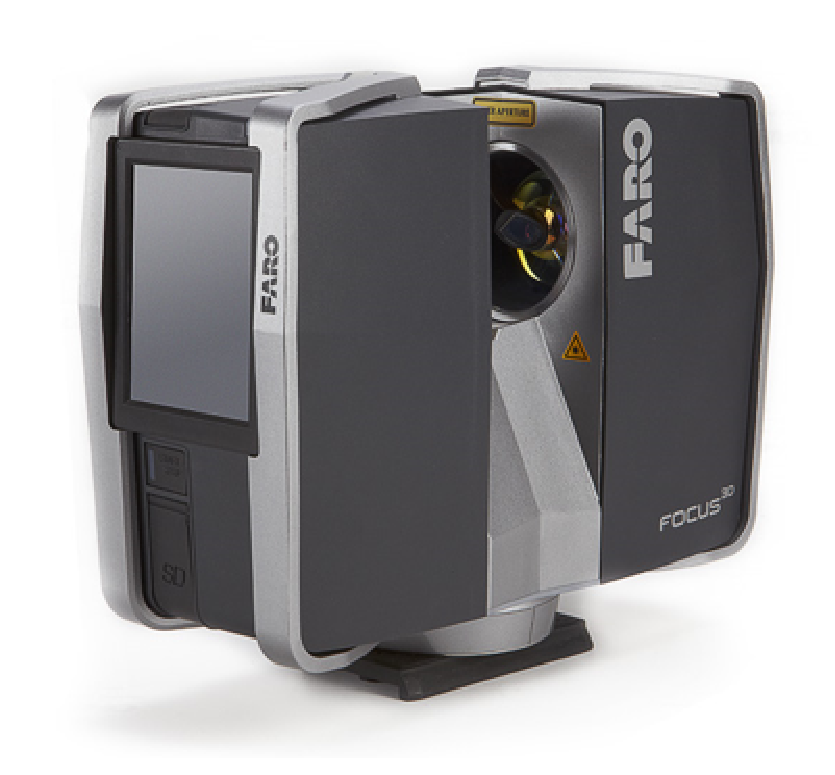
\includegraphics[height=70mm]{figure/FARO.eps}
   \caption{FARO Focus 3D}
   \label{FARO}
  \end{center}
\end{figure}

FAROのパラメータを設定してスキャンデータを撮ると,位置同定プログラムを動かすためにPTX形式に変える必要がある.スキャンデータをPTX形式に変えるときはSCENEというソフトを使う.SCENEはFAROで撮ったスキャンデータを可視化,色々な形式にエクスポート,その以外にも様々な機能がある.図3.17に解像度1/5,品質x2の地図データの例を表す.また,図3.18にはボクセル化された地図データの例を表す.

\begin{figure}[htbp]
  \begin{center}
   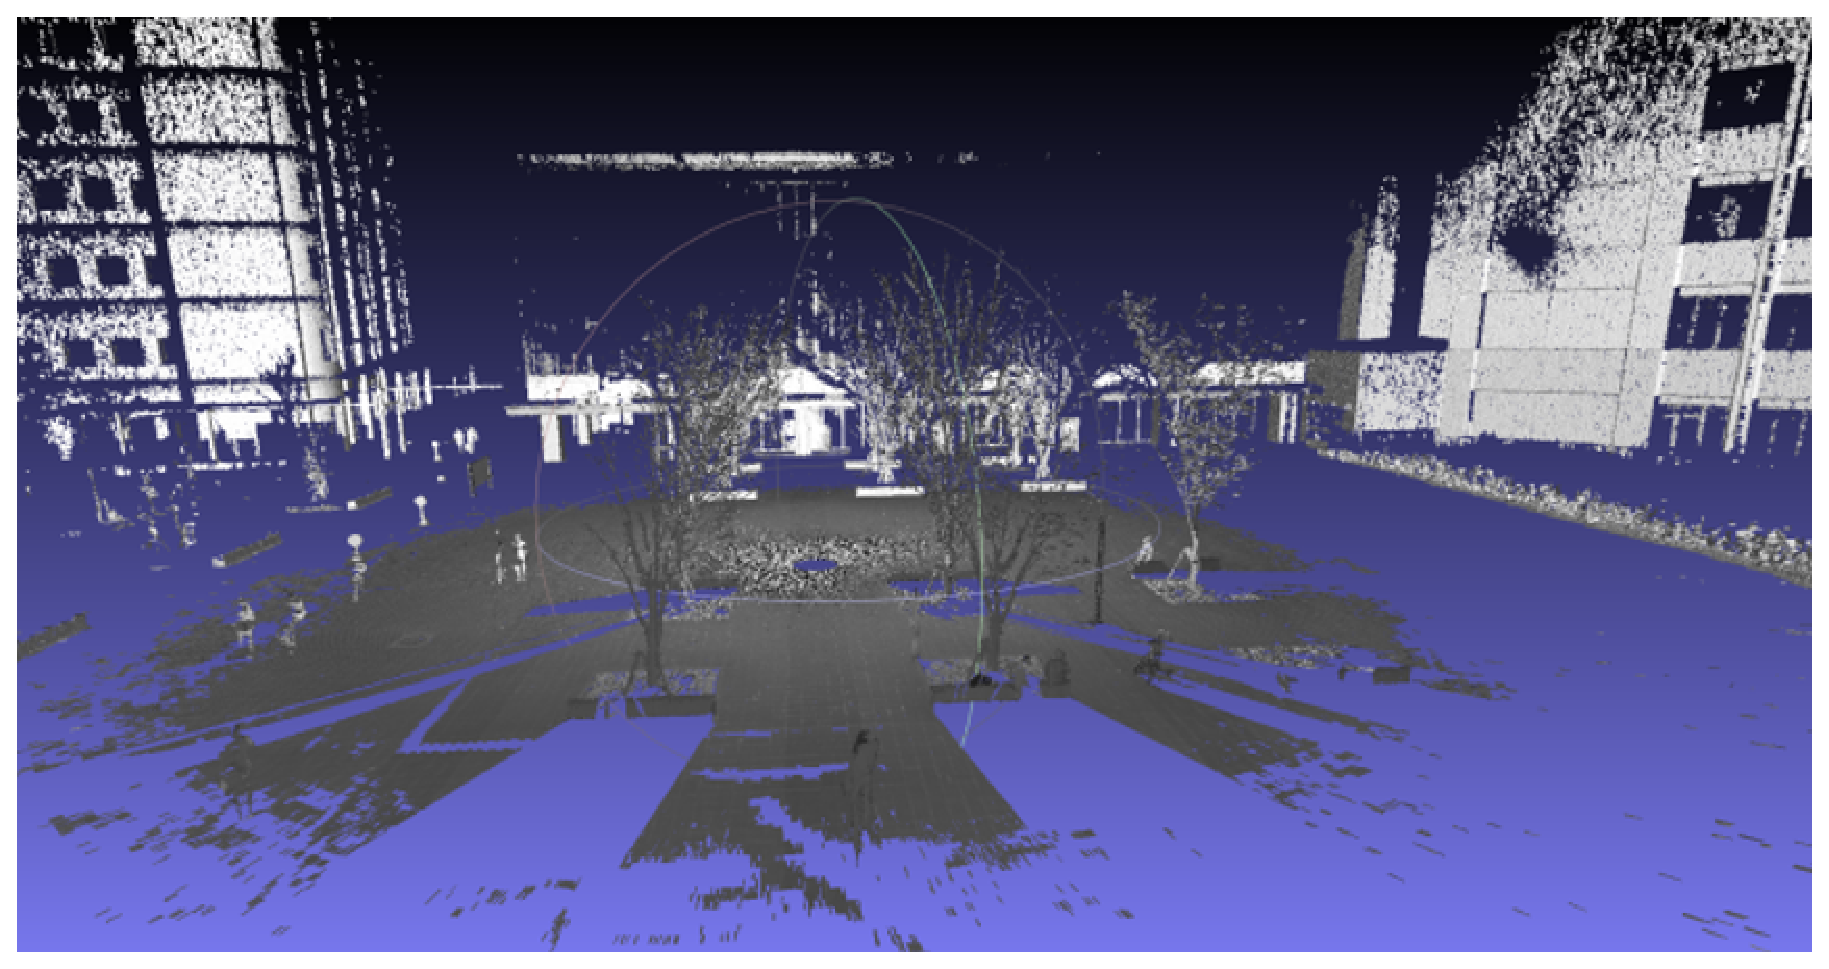
\includegraphics[height=80mm]{figure/地図データ(PTX).eps}
   \caption{地図データ(PTX)}
   \label{地図データ(PTX)}
  \end{center}
\end{figure}

\begin{figure}[htbp]
  \begin{center}
   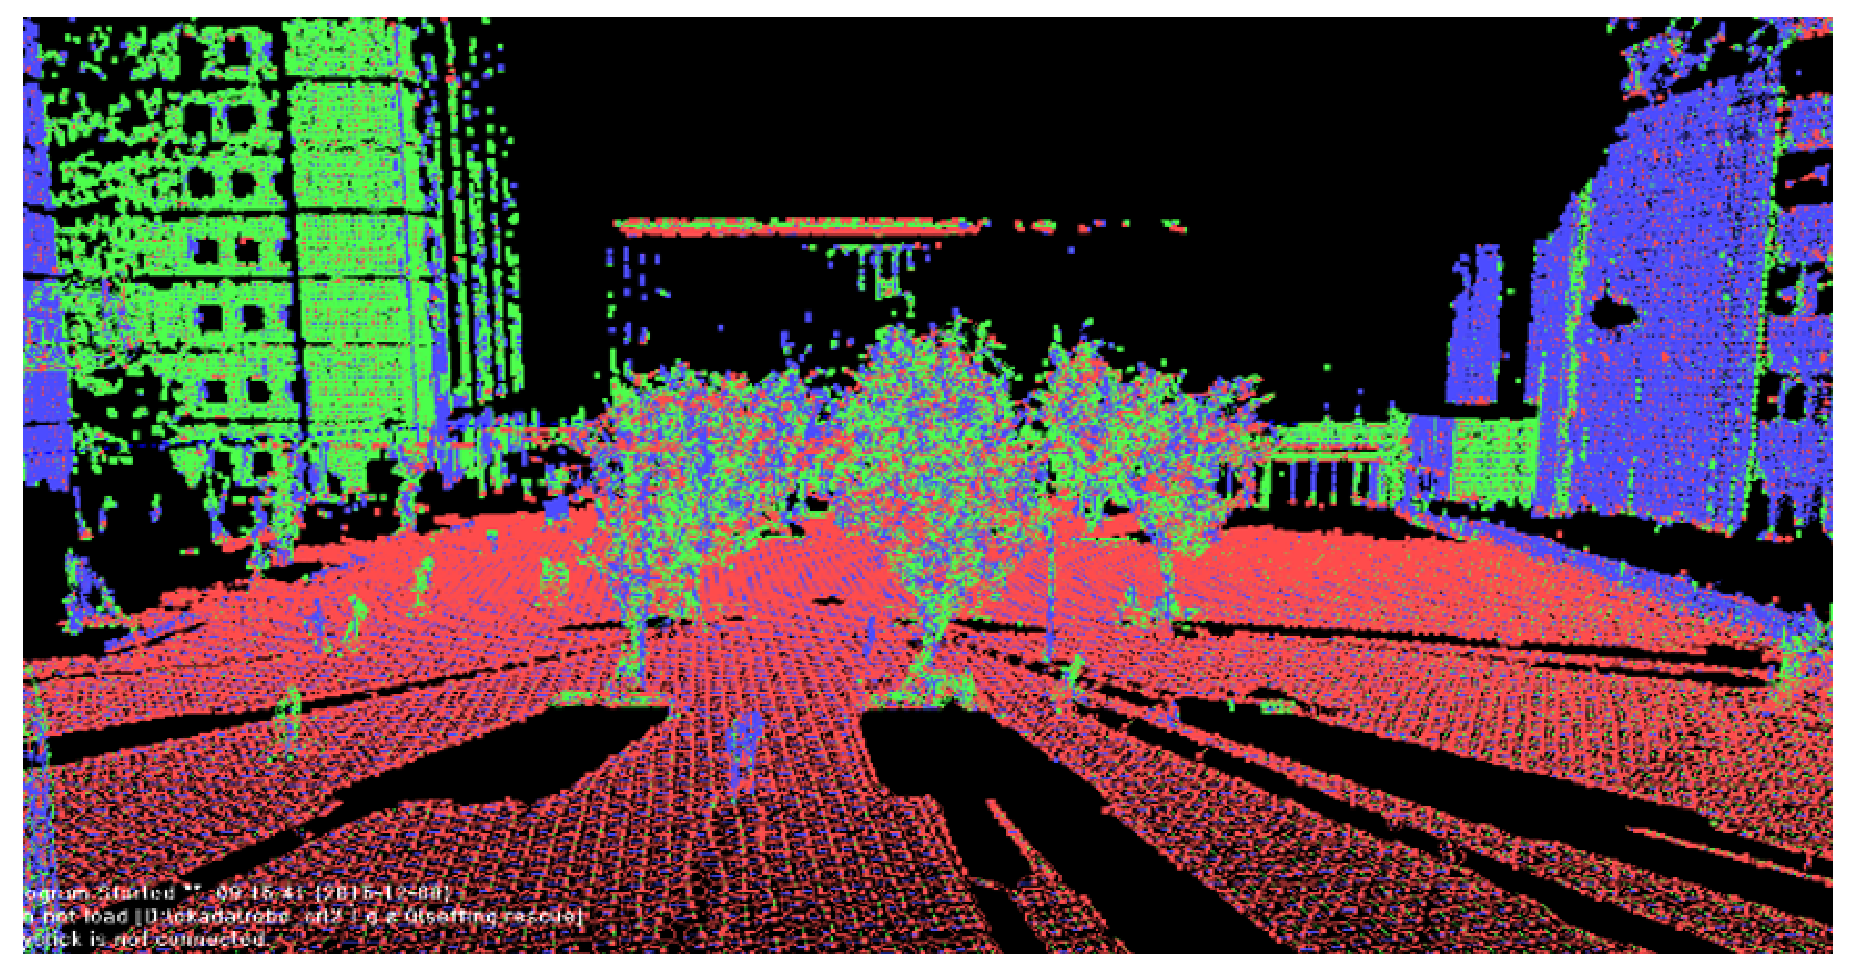
\includegraphics[height=80mm]{figure/地図データ(Voxel).eps}
   \caption{地図データ(Voxel)}
   \label{地図データ(Voxel)}
  \end{center}
\end{figure}

\vspace{15mm}
データの真ん中を見ると丸い穴があるが,これはFAROが実際置かれたところでFAROの真下が撮れていないため表れる死角である.撮れた地図データは前述の通り,SCENEソフトを用いてPTX形式化することで位置同定プログラムを動かす際の地図データができる.

\subsection{台車の位置計測法}

地図データと計測データを用いて位置同定を行い,パーティクルフィルタのリサンプリング100回目の収束位置を推定された位置とする.ただし,位置同定精度の性能を比較するためには,台車の位置計測値が必要となる.そこで,本章では台車の位置計測法について述べる.\par
まずは,地図データを撮ったFAROの位置で電源をONにしたまま,計測データを撮る台車を撮る.電源をONしたまま,続いて台車の位置を撮る理由は,FAROは電源の切り替えにより,FAROのX,Y座標軸が変わるからである.前述の通り,ステレオカメラの上に球を載せる理由は台車の位置計測ためと述べたが,SCENEソフトを用いると球の認識ができ,SCENEソフト上で球の座標値が分かる.SCENEソフトで球を認識し,座標値を出したキャッチャーを図3.19に表す.図3.19の右側のPositionというところに球の座標値が出る.

\begin{figure}[htbp]
  \begin{center}
   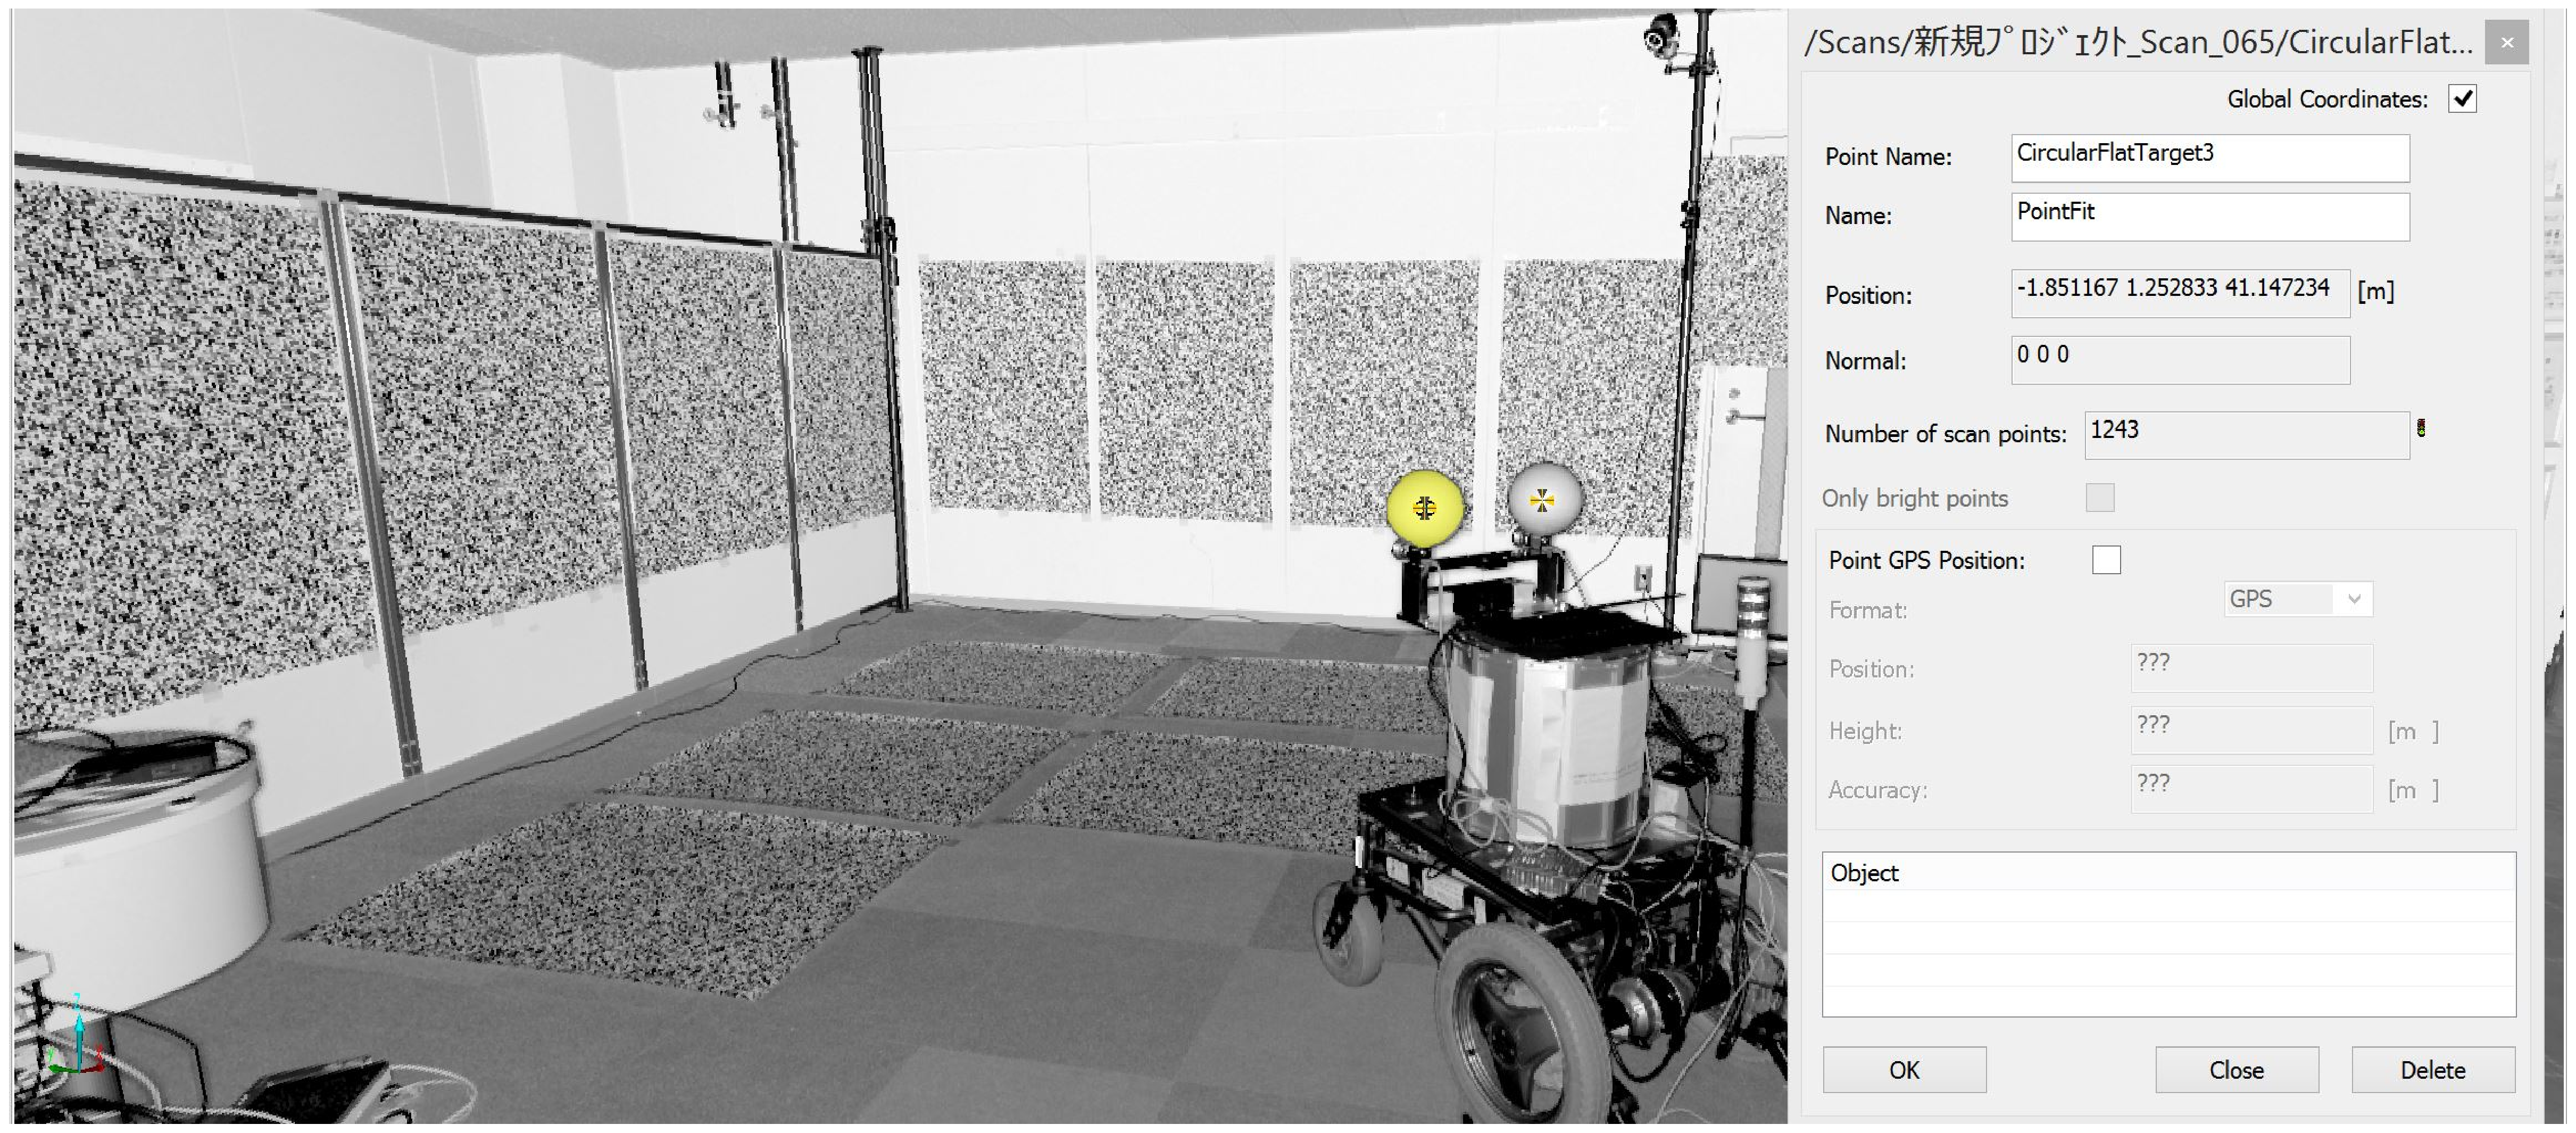
\includegraphics[height=70mm]{figure/球の認識.eps}
   \caption{球の認識}
   \label{球の認識}
  \end{center}
\end{figure}
\newpage

左右のステレオカメラの球座標から球の半径をZ軸に引いた値がステレオカメラの座標値となる.左のステレオカメラの座標値が計測データの真値となる.右ステレオカメラの球は左のステレオカメラの真値との計算を通して,方向を求めるために用いられる.つまり,計測データを撮る際はFAROからステレオカメラの上にある球が重ならないように注意するべきである.左ステレオカメラの座標値を($X_{l}$,$Y_{l}$,$Z_{l}$),右ステレオカメラの座標値を($X_{r}$,$Y_{r}$,$Z_{r}$)とすると,ステレオカメラの方向$D_{s}$は以下のように求められる.後,FAROから台車計測時の注意を図3.20に表す.

\begin{equation}
D_{s} = -1*\cfrac{X_{r}-X_{l}}{Y_{r}-Y_{l}} = \cfrac{X_{l}-X_{r}}{Y_{r}-Y_{l}}
\end{equation}

\begin{figure}[htbp]
  \begin{center}
   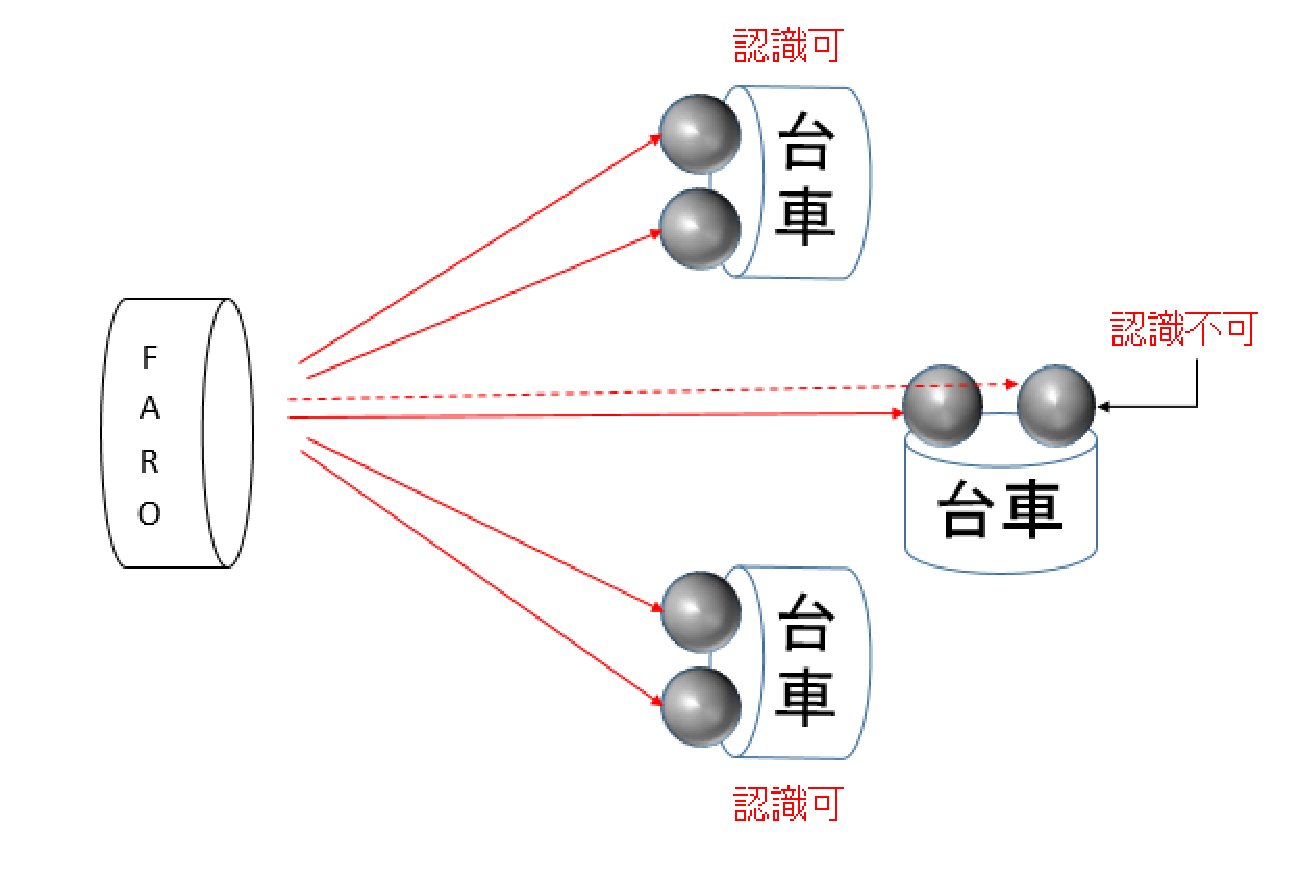
\includegraphics[height=70mm]{figure/撮影注意.eps}
   \caption{撮影注意}
   \label{撮影注意}
  \end{center}
\end{figure}

%---------------------------------------------------------------------------------------------------
